%!TEX TS-program = xelatex
%!TEX root = ../../maxwell2018thesis.tex

\chapter[A Background of Stopping in IIR]{A Background of Stopping in\\Interactive Information Retrieval}\label{chap:stopping_background}

In the previous chapter, we provided a high level overview of~\gls{acr:ir}. In particular, we provided a brief history of the area, the basic families of retrieval models, and various measures that have traditionally been used to evaluate the effectiveness of a retrieval system. Towards the end of the chapter, we began to shift from the \emph{system-sided} research that has dominated~\gls{acr:ir} research (and quite understandably so), towards the more \emph{user-centred} research with which the work in this thesis considers. In particular, as alluded to in Chapter~\ref{chap:intro}, and indeed in the title of this thesis, we now turn our attention to the concept of \emph{stopping behaviour} in the context of~\gls{acr:iir}.

\begin{figure}[h]
    \centering
    \vspace{4mm}
    \resizebox{1\hsize}{!}{
    
\includegraphics{figures/ch3-stopsign.pdf}}
    \label{fig:stopsign}
    \vspace{-5mm}
\end{figure}

With many of the models and measures employed in~\gls{acr:ir} and~\gls{acr:iir} research today largely agnostic of a searcher's stopping behaviour, we in this chapter provide an overview of a variety of different \emph{stopping heuristics} that have been defined in the literature over a number of decades, provide a discussion on a number of different user studies that have examined searcher stopping behaviours, discuss basic theoretical frameworks that provide a potential insight and explanation into why people stop, and then discuss a variety of different user models that have been developed that better attempt to model a searcher's interactions, and thus allow for a better representation of their stopping behaviour.

\section{Why Stopping?}
As previously mentioned, knowing when to stop is a fundamental aspect of human thinking and behaviour. Humans and other animals when interacting with the world will employ some form of \emph{stopping criterion} to decide when they should stop~\citep{nickles1995judgment}. As an example, a shopper who is looking to purchase a new smartphone will stop shopping around once he or she has obtained sufficient information on what new smartphone to purchase. Once their case notes for a patient have been compiled, a medical doctor will then be in a position to diagnose the patient's ailment.

The decision of when to stop is not exclusively due to factors external to the decision maker, but rather from a series of \emph{internal, cognitive factors} of their thinking process~\citep{nickles1995judgment}. An individual who is hungry will stop eating once he or she is no longer hungry, rather than stopping when all of the food presented to him or her has been consumed. Empirical research has over the years demonstrated that individuals, regardless of the task presented to them, will frequently stop prematurely. Indeed, this na\"{i}ve behaviour demonstrates that individuals may be willing to go with what \emph{``sounds right''} to them -- often minimising the cognitive effort that is required at the expense of greater accuracy~\citep{perkins1983difficulties}. However, this lower level of potential accuracy does lead searchers to making a greater number of errors in their decision making~\citep{baron1988heuristics}, with individuals overlooking important elements, and potentially miss out useful information~\citep{fischhoff1977cost_benefit, fischhoff1978fault, shafir1992thinking}, with the individual then failing to consider alternatives~\citep{farquhar1993decision_structuring}.

Based upon prior research into the phenomenon of stopping behaviour, it is clear that this is driven primarily from internal factors. As such, we then consider: \emph{what aspects of the decision maker's thinking processes prompt him or her to stop assessing the information provided?} Knowing when to stop requires that the individual in question makes a \emph{judgement} regarding the sufficiency of the information obtained, and whether or not additional information is required to be obtained~\citep{browne2004stopping_rules}. This judgement is normally characterised by both the completeness and correctness of the information obtained thus far~\citep{smith1991belief}. These claims can be mirrored by qualitative studies on examining stopping behaviour, where researchers have found that searchers stop examining a ranked list of results simply because what they have found previously is \emph{``good enough''}~\citep{zach2005enough_is_enough}, echoing the reasoning that individuals will be happy to stop when what they have found \emph{``sounds right''}~\citep{perkins1983difficulties}.

\section{Stopping Heuristics}\label{sec:stopping_background:heuristics}
Considering the above, researchers have over a number of decades devised a number of different high level \emph{stopping rules} -- hereafter referred to as \emph{stopping heuristics} -- as a means of encoding a searcher's aforementioned sense of what is \emph{``good enough''} -- or, indeed, what can be considered to be \emph{not good enough,} too.

Stopping heuristics have been investigated in \emph{decision making} research. A number of normative stopping heuristics have been identified. As examples of such heuristics,~\cite{busemeyer1988deferred_decision_making} considered the expected loss from terminating information acquisition.~\cite{kogut1990sunk_costs} examined the expected value of additional information. Other examples of normative stopping heuristics are demonstrated by~\cite{pitz1969information_seeking} and~\cite{busemeyer1988deferred_decision_making}. However, as outlined by~\cite{browne2004stopping_rules}, these heuristics usually fail to describe the actual cognitive behaviours of the decision makers. Such heuristics often assume that the decision maker must \emph{think ahead} to the final decision of when to stop, enabling them to assess the value of additional information~\citep{busemeyer1988deferred_decision_making}. This is however an inherently difficult task for decision makers to undertake, due to the limited working memory capacity of a human -- we are simply unable to hold and evaluate all of the information attained to make a decision considering all possible outcomes~\citep{browne2004stopping_rules}.~\cite{nickles1995judgment} agreed, stating that normative stopping heuristics made implicit assumptions about the mental activities of the decision maker, especially in terms of mental scaling and weighting. No clear cognitive perspective is provided to address the assumptions of the decision maker's thinking.

With these inherent limitations in mind, seminal work in this area was undertaken by~\cite{nickles1995judgment} who provided a broad classification for different explicitly defined stopping heuristics in the literature that consider a searcher's cognitive processes: \emph{judgement based heuristics} and \emph{reasoning based heuristics.} These were devised largely as ways of modelling the \emph{Expected Search Length}~\citep{cooper1968expected_search_length}, as described in Section~\ref{sec:ir_background:evaluation:esl}.~\cite{nickles1995judgment} also proposed a number of stopping heuristics that are discussed in subsequent sections, with discussion expanded to included additional heuristics defined by other researchers.

\subsection{Judgement Based Heuristics}
A judgement based stopping heuristic is defined as when a decision maker is assumed to set and consistently maintain a mental threshold along some form of key dimension (e.g. determining the seemingly relevant from non-relevant), and to keep a running total of measure relative to the dimension in question~\citep{gettys1979hypothesis, nickles1995judgment}. When the measure is met or exceeded this set threshold, the searcher then stops and proceeds to the next step, or abandons the search altogether. A number of different judgement based heuristics have been defined in the literature, the most prominent of which we discuss here.

\subsubsection{Satisfaction and Frustration}\label{sec:stopping_background:heuristics:judgement:satisfaction_frustration}
Two of the earliest stopping heuristics defined in the literature are by~\cite{cooper1973retrieval_effectiveness_ii} which consider a searcher's tolerance to relevant and non-relevant material. The heuristics were originally defined as a means for estimating the utility a searcher can attain when interacting with a search system. While the means of which~\cite{cooper1973retrieval_effectiveness_ii} estimated the utility of search are not of key relevance to this thesis, the work on stopping heuristics are. The \emph{satisfaction point} and \emph{frustration point} stopping heuristics are considered to be judgement based heuristics, as they rely solely on the searcher's notion of what constitutes a relevant document -- and both consider counts of the number of (non-)relevant documents observed.

\noindent\blueboxbold{Satisfaction Point}
Given the name, it is not surprising that the \emph{satisfaction point} rule considers the point at which a searcher has found enough perceived relevant material to consider his or her search a success. It can be easily imagined that such a rule would apply directly to both snippet level stopping (i.e. \emph{find $x$ relevant documents on this SERP}) and session level stopping (i.e. \emph{find $x$ relevant documents}). This heuristic is also called the \emph{satiation heuristic} (see below). This heuristic can be considered as a decision making process...

\begin{quote}
    \emph{``through which an individual decides when an alternative approach or solution is sufficient to meet the individuals' desired goals rather than a perfect approach.''}
    \attrib{\cite{simon1971decision}}
\end{quote}

This essentially suggests that a searcher employing this particular heuristic would stop searching as soon as certain conditions arise, instead of after they have exhaustively considered all available information~\citep{march1994primer}. Conditions could include acceptance of the results, discomfort, boredom, time limits and the \emph{snowballing} of information~\citep{mansourian2007search}.

\noindent\blueboxbold{Frustration Point}
In a converse fashion to the satisfaction point heuristic, the \emph{frustration point} heuristic considers a searcher's overall \emph{tolerance to non relevance}, by stopping after being sufficiently frustrated by the results presented to the searcher. This heuristic is also called the \emph{disgust heuristic} in the literature (see below).

The two relatively straightforward heuristics defined above makes a searcher's interactions with a ranked list of results, or SERPs, \emph{inherently adaptive.} Given a set of results, his or her behaviour will change with respect to the perceived quality of the ranked list of results. As a reminder, this would not necessarily mean considering the system's effectiveness measures, but rather user-focused measures such as interactive precision and recall (refer to Section~\ref{sec:ir_background:user:evaluation:interactive_pr}).

\noindent\blueboxbold{Combining Satisfaction and Frustration}
Perhaps due to the relative simplicity of these heuristics, identical approaches have also been defined elsewhere in the literature.~\cite{kraft1979stopping_rules} later defined three further stopping heuristics, two of which are the \emph{satiation} (as per~\cite{simon1955satiation}) and the somewhat loaded \emph{disgust} heuristics. In essence, the rules defined by~\cite{kraft1979stopping_rules} are the same satisfaction and disgust heuristics as previously defined by~\cite{cooper1973retrieval_effectiveness_ii}. Within the satiation rule, a searcher will stop after been \emph{satiated} by finding a number of documents considered to be relevant, while the disgust rule considers a searcher's disgust at finding a number of non-relevant documents.

\cite{kraft1979stopping_rules} also proposed a third heuristic that \emph{combines} both the satisfaction/satiation and frustration/disgust rules together into a single heuristic. Here, a searcher following such an approach would be inclined to stop examining content if they were either satisfied with what had been found, or frustrated by having to trawl through a number of material judged to be non-relevant. The stopping point would be whatever of the two conditions are met first. Indeed,~\cite{kraft1979stopping_rules} demonstrated that the expected search length of a searcher could be approximated using each of the two stopping heuristics by considering the size of the retrieval set, the number of relevant documents a searcher wished to obtain, and the number of non-relevant documents a searcher would be willing to tolerate. The number of documents required to consider a search as successful is dependent upon whether the search task is high precision (where one would stop comparatively early), or high recall (where one would stop comparatively later), as hypothesised by~\cite{bates1984thirty_items}.

\subsubsection{Magnitude Threshold}\label{sec:stopping_background:heuristics:judgement:magnitude}
The magnitude threshold heuristic, as outlined by~\citep{nickles1995judgment}, considers an individual's belief that the information accrued during the search process provides sufficient \emph{evidence} to prompt him or her to stop searching for information. The point at which the searcher would decide to stop is determined by some predetermined, internal threshold that must be reached, which acts as the stopping criterion~\citep{wald1948sequential_analysis, nickles1995judgment}.~\cite{gettys1979hypothesis} hypothesise that the searcher \emph{`mentally tabulates'} the cumulative impact of the evidence that he or she has uncovered, and when the internal tabulation crosses the specified threshold, he or she stops.

\begin{wrapfigure}{r}{0.45\textwidth}
    \begin{center}
    \vspace*{-10mm}
    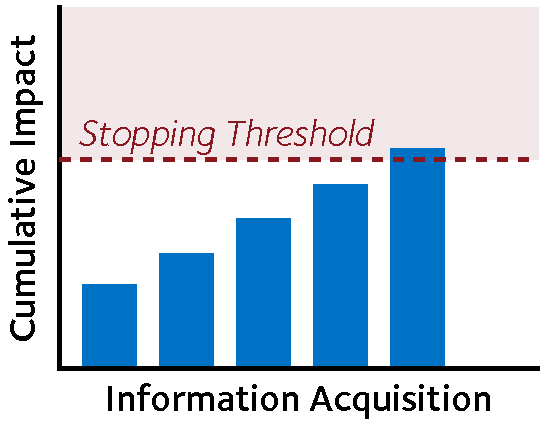
\includegraphics[width=1\textwidth]{figures/ch3-threshold.pdf}
    \end{center}
    \vspace*{-4mm}
    \caption[The magnitude threshold stopping heuristic]{The magnitude threshold stopping heuristic. Once a searcher accrues a predetermined level of impact, he or she stops. Figure adapted from~\cite{browne2004stopping_rules}.}
    \label{fig:threshold}
\end{wrapfigure}

Determining what exactly this threshold should be before commencing a task has attracted research from several perspectives. Indeed, this decision can be left open to interpretation by the individuals who choose to operationalise such a heuristic. However, research has shown that under different tasks, varying the criteria by which an individual bases their initial threshold value varies. For example,~\cite{busemeyer1982choice_behaviour} demonstrated this for decision making under uncertainty.~\cite{saad1996stopping} demonstrated the usefulness of this heuristic under common choice tasks.

An abstract representation of the stopping heuristic is provided in Figure~\ref{fig:threshold}. From the figure, we can see that a searcher accrues information through each document that is examined. This is combined together to form a \emph{cumulative impact} for the information. For each document examined, the current cumulative impact value is compared against a predetermined threshold value -- if the cumulative impact appears to be above the threshold, the searcher then assumes that enough supporting evidence has been collected, and subsequently stops.

\subsubsection{Difference Threshold}\label{sec:stopping_background:heuristics:judgement:difference}
Again outlined by~\citep{nickles1995judgment}, the \emph{difference threshold heuristic} concerns whether a new document is teaching a searcher anything new about their given information need, or the marginal value of the latest document. Here, the searcher is assumed to keep an internal record of the cumulative impact of information that has been consumed along some key dimension. The searcher is also assumed to use this internal record of what has been assessed to compare a new document with previously examined content. When the absolute difference between the two assessments falls below some internal difference threshold, the searcher would then stop as nothing new is being learnt.

\begin{figure}[t!]
    \centering
    \resizebox{1\hsize}{!}{
    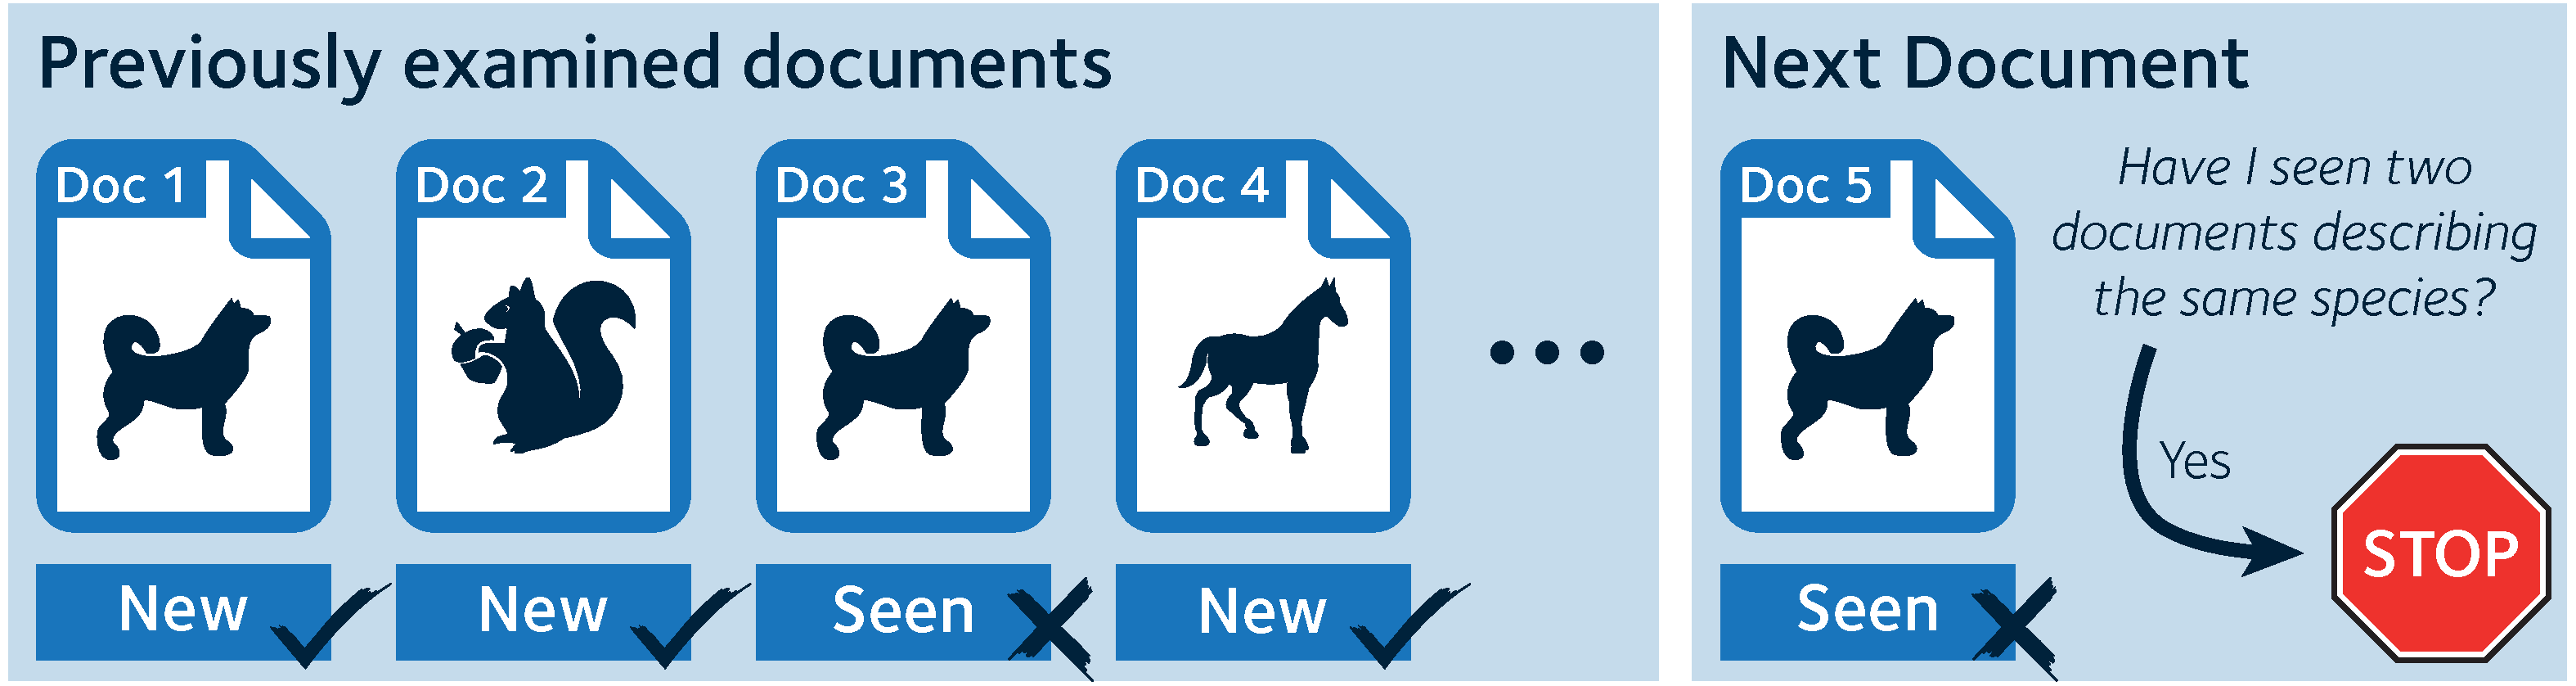
\includegraphics{figures/ch3-difference.pdf}}
    \caption[Difference threshold heuristic]{A simplified, visual example of the difference threshold heuristic. Given the information need of finding different species of animal, a searcher issues a query, and examined a number of documents. The third document offers information on dogs, which has been already observed in \blueboxbold{Doc 1}. Using the stopping criterion that once the same species has been observed twice, \blueboxbold{Doc 5} satisfies it – and thus, the searcher stops.}
    \label{fig:difference_heuristic}
\end{figure}

As a crude example of this heuristic, a searcher is provided with an information need to find as many different species of animal as possible. Once a query has been issued, the searcher begins to examine documents on the SERP. This is illustrated in Figure~\ref{fig:difference_heuristic}, where the first document considers dogs. A simple criterion is employed whereby the searcher stops after encountering the same animal twice, illustrating that nothing new is being learnt from the list of results presented. Once this is met, the searcher abandons the SERP, and can then perform a query reformulation to discover different species of animal.

\subsubsection{Single Criterion}
The \emph{single criterion heuristic} was later defined by~\cite{browne2005stopping_rules}. As the name suggests, this heuristic considers a searcher examining information for a \emph{single criterion} related to their information need, typically assumed to be the most important one. The searcher then stops examining content once he or she has deduced that enough information about said criterion has been accumulated for them to be satisfied. The concept of a stopping threshold can be borrowed from the magnitude threshold heuristic. This considers that a searcher will stop once they have accumulated enough impactful information.

\cite{browne2005stopping_rules} go on to provide an example search task where the single criterion threshold would be directly applicable. When purchasing a mortgage for a new house, a searcher will explore various mortgage lender's websites in order to find the best deal. Given a mortgage deal, the most obvious criterion that an individual would look for would be interest rates -- the lower, the more attractive the deal. Of course, other factors may influence the decision, but this example ultimately demonstrates a potential application of the heuristic.

\subsection{Reasoning Based Heuristics}
The second category of stopping heuristics as defined by~\citep{nickles1995judgment} are \emph{reasoning based}. While searching and accruing information about a particular topic, a searcher is essentially developing a form of mental representation of the various elements of the topic as he or she learns~\citep{yates1990decision_making}. As argued by~\citep{nickles1995judgment}, these elements can include arguments constructed during informal reasoning, previously constructed arguments, or information evoked from the searcher's long term memory. As such,~\citep{nickles1995judgment} devised a category of stopping heuristics that are dominated by the searcher's reasoning processes.

\subsubsection{Representational Stability}\label{sec:stopping_background:heuristics:reasoning:representational}
\begin{wrapfigure}[8]{r}{0.45\textwidth}
    \begin{center}
    \vspace*{-10mm}
    
\includegraphics[width=1\textwidth]{figures/ch3-representational.pdf}
    \end{center}
    \vspace*{-4mm}
    \caption[Representational stability stopping heuristic]{A crude illustration of the representational stability stopping heuristic. The searcher's model of the given information need begins to stabilise at \emph{t-1}, meaning that a searcher would stop at \emph{t}.}
    \label{fig:representational_heuristic}
\end{wrapfigure}

This heuristic concerns the notion that as a search acquires new information via the search process, his or her mental model of the underlying information need shifts and develops -- but only up to a certain point. From this point where their mental model stabilises, the searcher is said to have accrued enough information to satisfy their information need.

The notion of representational stability is based upon the stopping heuristic outlined by~\cite{nickles1995judgment}, the phenomenon of which is initially discussed by~\cite{yates1982toward}.~\cite{nickles1995judgment} argues that while a searcher examines content, he or she generates arguments that serve to develop and elaborate his or her conception of the decision(s) that they are tasked to make. As the searcher continues to reason, certain arguments may be relegated to long term memory due to the limited size of the searcher's working memory. As the information seeking process continues, constructs arguments from this information and accommodates his or her mental model of the information need, the searcher may at some point return to the same subset of arguments. As mentioned previously, it is at this point that can be interpreted as a form of stability regarding the information need. This is crudely demonstrated in Figure~\ref{fig:representational_heuristic}, where given a vague information need, a searcher will trawl a series of documents in order to develop their mental model of the given problem.

\subsubsection{Propositional Stability}
Similar to the representational stability heuristic,~\cite{nickles1995judgment} also defined the \emph{propositional stability} heuristic again focuses on the concept of a stabilising mental model of the given information need. Here, a searcher when examining content will form a series of arguments from the information he or she is observing. These arguments can lead to \emph{tentative conclusions}, from which at some point stability is achieved, and the conclusion does not change. This heuristic therefore suggests that the stabilised nature of the decision maker's conclusion from the information observed prompts him or her to stop.

\subsubsection{Mental List}
This final reasoning based stopping heuristic concerns the notion of a searcher constructing a mental list of items or aspects of a particular item that they are attempting to search for. Each of the different items within the mental list must be checked off to a satisfactory level before the searcher then decides to stop examining content. This mental list can typically be constructed from a searcher's long term memory -- meaning that they will likely have \emph{a priori} knowledge of the particular information need. So-called belief structures such as \emph{schema}~\citep{bartlett1933remembering} or \emph{scripts}~\citep{schank1977scripts} may assist the searcher in organising the construction of the mental list that will form the set of criteria that determines when they stop.

Figure~\ref{fig:mental_list} provides a graphical illustration of the mental list heuristic. When looking for a new car, a searcher will construct a mental list of different aspects of a car which are essentially the minimum requirements (e.g. a minimum engine displacement of 1.8 litres). Searching is then conducted, with the searcher narrowing down the potential choices available to them to those that satisfy their mental list.

\begin{figure}[t!]
    \centering
    \resizebox{1\hsize}{!}{
    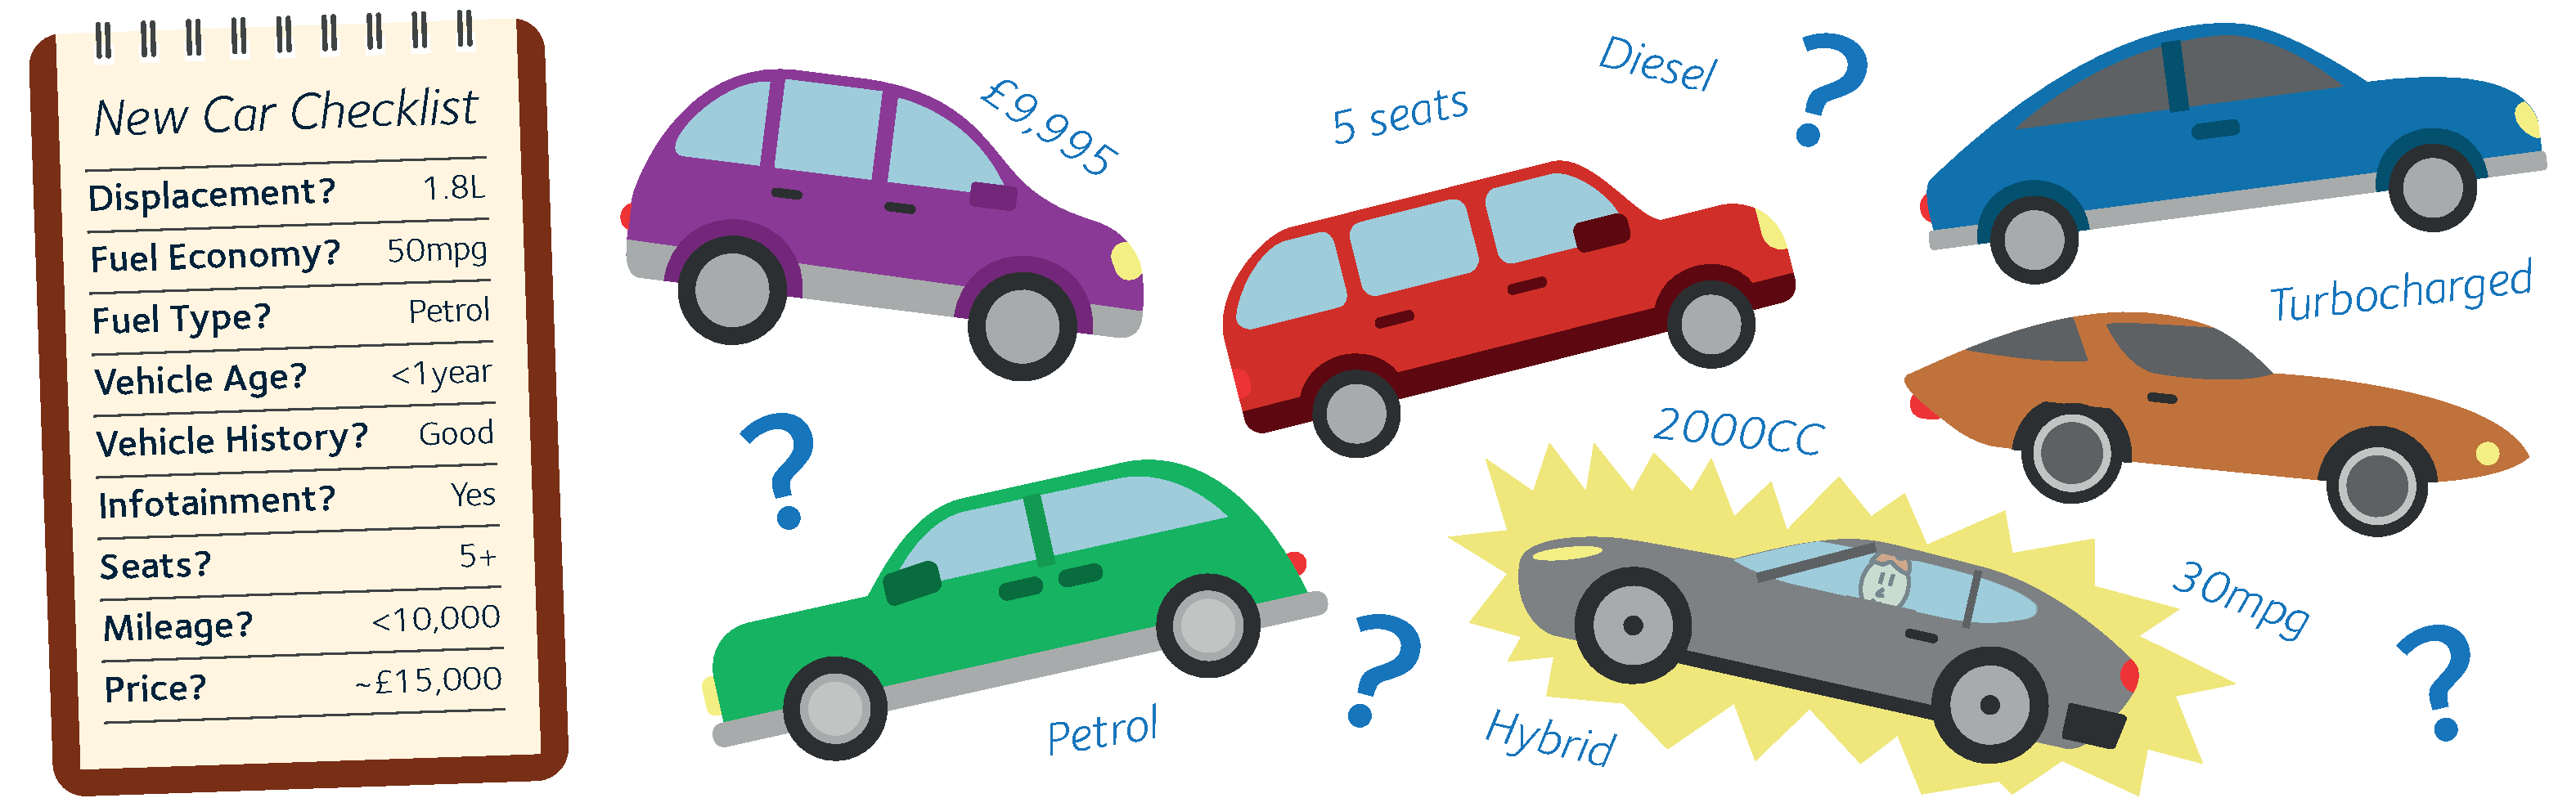
\includegraphics{figures/ch3-mental_list.pdf}}
    \caption[The mental list stopping heuristic]{Given a well defined information need,~\cite{nickles1995judgment} defined the mental list heuristic – where a number of different criteria must be satisfied before stopping. In the illustration above, car shopping is used as an example. Here, certain criteria for a new car (as shown on the notepad) must be met before a searcher is satisfied with what they have found.}
    \label{fig:mental_list}
\end{figure}

\subsection{Summary of Heuristics}
In this section, a number of different stopping heuristics have been discussed from a number of seminal papers in the literature. While a much larger of number of normative stopping heuristics have been defined in prior works, these have been omitted from the review as they do not adequately describe the cognitive behaviours of a searcher, often assuming a searcher has to \emph{think ahead} to make a decision to stop or continue~\citep{browne2004stopping_rules}. In contrast, the heuristics that are enumerated above do not make this assumption, making more realistic assumptions about the searcher's cognitive abilities.

Of course, the different stopping heuristics discussed above are likely to behave differently under different search contexts. As an example, the mental list heuristic might be impossible to use given a searcher with a very limited knowledge of a topic. He or she simply would not know enough information to ascertain key aspects of the topic, and construct a set of criteria that must be met~\citep{browne2005stopping_rules} --~\cite{gigerenzer1999betting} also discuss this reasoning for the single criterion heuristic. As such, it is hypothesised that the aforementioned stopping heuristics would be likely to work better with a searcher who is more knowledgeable. Indeed,~\cite{browne2005stopping_rules} hypothesises that magnitude threshold and mental list heuristics would be best applied to searchers with a greater degree of understanding of the topic.

\cite{browne2005stopping_rules} also discuss the so-called \emph{``structuredness''} of a given search task. If the task has well defined inputs and outputs -- or the goals and operations are clear and easily understood~\citep{simon1996sciences} -- then it it hypothesised that searchers will employ more precise stopping heuristics for deducing when to stop. For example, the mental list and single criterion stopping heuristics might offer greater degrees of precision than for example the frustration and satisfaction heuristics, although the frustration and satisfaction heuristics may perform well for any given search task. Altogether however, the heuristics discussed in this section would all be applicable for information search~\citep{browne2005stopping_rules}.

With the heuristics now enumerated, we later in this thesis discuss how we take the heuristics, and consider how to \emph{operationalise} them, such that they can be subsequently implemented and compared against each other in an empirical way. Refer to Section~\ref{sec:proposal:strategies} for the complete set of \emph{stopping strategies} that we employ.

\section{User Studies}\label{sec:stopping_background:user_studies}
While stopping heuristics provide a means for quantitatively characterising and predicting stopping behaviour~\citep{wu2014information_scent}, only a handful of user studies have been undertaken that attempt to understand what the aforementioned sense of what is \emph{``good enough''}~\citep{zach2005enough_is_enough} actually entails. This is not necessarily surprising. As we have already discussed, stopping is an inherently difficult phenomenon to model effectively -- this is because it is instrumented by a series of internal factors to the decision maker's thinking~\citep{nickles1995judgment}. But what are these internal factors? In this section, we detail a number of different user studies that have attempted to provide an explanation for a searcher's stopping behaviours.

\subsection{Understanding Stopping Behaviours}
%\todo{Satisficing offers a framework~\citep{toms2009predicting_stopping} ~\cite{simon1955satiation}, considering bounded rationality}

As reported by~\cite{wu2014information_scent}, a majority of user studies that examine stopping behaviours have been conducted as a series of interviews. These studies primarily focused on the notion of \emph{why} searchers stopped when they did.

For example, two prominent studies in this area were conducted by~\cite{zach2005enough_is_enough} and~\cite{berryman2006defines}. In these studies, stopping behaviour in academic work environments were studied. The study by~\cite{zach2005enough_is_enough} considered how senior art administrators determined when to stop searching in their daily jobs, and found that they mostly stopped either because they either: \emph{(i)} felt satisfaction with the information that they had obtained during their search; or \emph{(ii)} stopped because of time constraints.~\cite{berryman2006defines} conducted a study along a similar vain, where public sector policy workers reported finding it difficult to work out how much information would be enough to satisfy their tasks when initiating them. However, once the structure of what they needed to find has been established, the point at which they felt they should stop became clearer. The findings from this second study provide evidence that the assessments of what constitutes as \emph{enough} can be difficult and complex to deduce. This finding also provides evidence of the development of an underlying mental model of the given information need, and provides justification for stopping heuristics such as representational stability (refer to Section~\ref{sec:stopping_background:heuristics:reasoning:representational}).

% Summary:
% agosto2002satisficing - High School Students’ Information Seeking and Use for Class Projects -- Chung (2006)

A number of user studies have also examined stopping behaviour in relation to the concept of satisfaction or \emph{satiation}~\citep{simon1955satiation}. As previously discussed in Section~\ref{sec:stopping_background:heuristics:judgement:satisfaction_frustration}, this concept suggests that a searcher will cease searching as soon as conditions arise instead of after they have exhaustively considered all available information~\citep{march1994primer}. Considering this approach,~\cite{agosto2002satisficing} examined the decision making of young people when searching on the~\gls{acr:www}. In this study, 22 9\textsuperscript{th} and 10\textsuperscript{th} grade students from a US high school demonstrated limitations which affected their decision making, including time constraints that were imposed externally and internally, information overload and other physical constraints. In order to find websites to help in satisfying their information need, the students used reductive approaches to decrease the amount of information presented on the~\gls{acr:www}, and used this to work out when to stop. How students perceived the websites was also largely down to personal preference. With a completely different set of subjects,~\cite{mansourian2007search} conducted a study where they analysed the stopping behaviours of 37 staff and students from four university biology departments, and classified their stopping behaviours by its search depth and search impact. Qualitative results showed that subjects indicated that missing potentially important information in the course of their searching was a matter of concern. The authors reported that the estimations and importance of information missed likely would affect their stopping behaviour. From this, classifications of the perceptions of missing information ranged from \emph{inconsequential} to \emph{disastrous}, and search strategies classified as \emph{perfunctory} to \emph{extensive}, with the information need dictating what category the searcher would have considered appropriate. A similar study by~\cite{prabha2007enough} considered searchers in a further academic library setting, with one key finding from their study showing that time constraints led to a decrease in the number of documents that searchers examined. Again, the specific information need and the searcher's role in academia affects every stage of their search processes -- which includes affecting what they have found to be enough.

This was further demonstrated by~\cite{wu2014information_scent}, who undertook a study where subjects performed a series of different search tasks. Subjects were then interviewed about their query stopping and task stopping behaviours. Results from this study showed that query stopping decisions were taken primarily on the face of search results, queries and search tasks. Task stopping decisions were determined by the subject's overall goal for each task, the content examined -- and their subjective perceptions of the examined content -- and the study constraints imposed upon them, such as time constraints and search interface restrictions. Further empirical evidence to this study was later provided by~\cite{wu2014stopping_query_abandonment}. They reported that some subjects discussed \emph{``forced stopping''}, stopping when no more information could be found, and \emph{``voluntary''} stopping that was the result from securing enough (or a necessary amount of) information.

\cite{wu2014information_scent} also discussed how the so-called \emph{information scent} affects the stopping behaviour of a searcher. Part of~\glsfirst{acr:ift} that we discuss in Section~\ref{sec:stopping_background:models:theoretical:ift}, it is important to note that user studies have been conducted using this approach. For example,~\cite{card2001scent_graphs} observed that if a person started with a high information scent web page, he or she would visit more web pages at the site. They also found that as the information scent of web pages declined, there was a tendency for the person to leave the site or return to a previously visited page. Scent was also examined by~\cite{loumakis2011image_smells} associated with images presented on~\glsplural{acr:serp} impacted with the evaluation behaviour of searchers. They found that when images were added to text snippets, participants reported increased confidence that they could find an answer.

Central to the findings of all of the above studies -- regardless of the group of subjects or contexts in which they found themselves to search in -- is the idea that searchers stop when they are \emph{satisfied.} Even though subjects of these studies were acutely aware of the fact they had not found \emph{all} relevant information to their given information need, they were nevertheless satisfied with what they had found, and subsequently decided to stop. While the results from these studies may be underwhelming in terms of concrete explanations as to why people do stop, they do provide invaluable insights -- and demonstrates just how difficult it is to encapsulate such behaviour. Indeed, factors such as time constrains, a searcher's information seeking ability and other factors all influence the internal stopping rules of a searcher, as was discussed by~\cite{marchionini1995information_seeking}. 

\subsection{Quantifying Stopping Behaviours}
With the above studies examining \emph{why} people decide to stop, a very limited number of studies have attempted to quantify \emph{when} a searcher should stop searching -- somewhat akin to the stopping heuristics defined in Section~\ref{sec:stopping_background:heuristics}.~\cite{toms2009predicting_stopping} studied the actions preceding the endpoints in information seeking to predict what actions would lead a searcher to stop. The most prevalent patten they observed consisted of a searcher:

\begin{itemize}
    \item[\emph{(i)}]{issuing a query;}
    \item[\emph{(ii)}]{examining results presented to them on a~\gls{acr:serp}; and}
    \item[\emph{(iii)}]{viewing a document.}
\end{itemize}

Interestingly, the authors observed that searchers appeared to be more engaged in page content and in revisiting and assessing pages that had already been found. They hypothesised that this again may be due to the satiation heuristic, where the searchers would purposefully go back to reassess if what they had found was \emph{enough.}

\begin{wrapfigure}[12]{r}{0.45\textwidth}
    \begin{center}
    \vspace*{-10mm}
    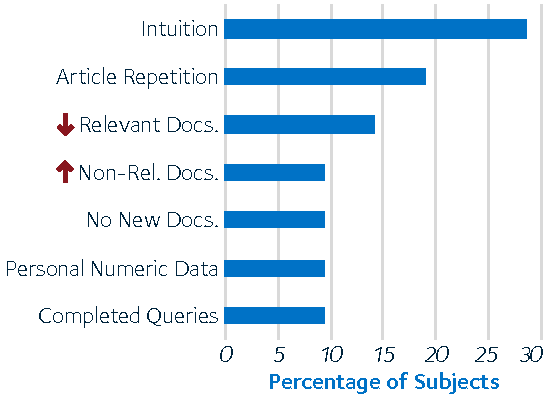
\includegraphics[width=1\textwidth]{figures/ch3-respondents.pdf}
    \end{center}
    \vspace*{-4mm}
    \caption[Responses of a survey by~\cite{dostert2009satisficing}]{Responses of the survey on why subjects stopped by~\cite{dostert2009satisficing}. Like most studies examining stopping behaviour, most subjects stopped because of their \emph{intuition.}}
    \label{fig:stopping_respondents}
\end{wrapfigure}

A further study by~\cite{dostert2009satisficing} examined the stopping behaviours of 23 undergraduate students. Subjects, like in other studies, reported that the primary factor for deciding to stop was their intuition. Again, subjects were time constrained --~\cite{dostert2009satisficing} reasoned that subjects could not adequately articulate this intuition, but hypothesised that they simply felt that given their perception of how much time had elapsed, the number of documents that they had located felt sufficient. The authors however report a number of additional reasons (as shown in Figure~\ref{fig:stopping_respondents}) why subjects decided to stop, with the reasons providing links back to the stopping heuristics defined in Section~\ref{sec:stopping_background:heuristics}.

Indeed, the unarticulated notion of finding \emph{``enough''} information links neatly back to the idea of the magnitude threshold stopping heuristic, proposed by~\cite{nickles1995judgment} and detailed in Section~\ref{sec:stopping_background:heuristics:judgement:magnitude}. With this heuristic, a searcher would stop once they have accumulated a certain, predetermined amount of information. From the results of their study,~\cite{dostert2009satisficing} hypothesised that the threshold was reached once they felt they had correctly identified \emph{half} of the relevant documents available to them. However, in reality, the searchers had on average only managed to correctly identify $7.35\%$. In addition to comparisons to the magnitude threshold stopping heuristic,~\cite{dostert2009satisficing} also drew comparisons from their results to the difference threshold stopping heuristic, as outlined in Section~\ref{sec:stopping_background:heuristics:judgement:difference}. Recapping, this heuristic considered a searcher's tolerance to not learning anything new -- this is argued by the authors as a reason for respondents citing repetition in the documents found, or a lack of new documents. Lastly, the representational stability stopping heuristic as detailed in Section~\ref{sec:stopping_background:heuristics:reasoning:representational} was also noted by the authors. With this heuristic concerned with the searcher's underlying mental model of the topic stabilising, the authors noted that evidence for this was shown from subjects responding that a decreasing in relevant documents and an increase in non-relevant documents.

These stopping heuristics were also investigated by~\cite{browne2004stopping_rules} and~\cite{pitts2004stopping_rules} with systems analysts during the process of information requirements determination. The analysts were tasked to gather a series of requirements until they had acquired enough information to draw diagrams of an online grocery shopping system. It was found by~\cite{browne2004stopping_rules} that more experienced analysts tended to use the mental list and magnitude threshold stopping heuristics, with less experienced analysts employing the difference threshold and representational stability stopping heuristics. In addition to these findings, the authors noted that the applicability of different stopping heuristics resulted in varying degrees of quantity, depth and the quality of information obtained.

\subsection{Considering Search Depths}
A number of additional user studies have also considered the so-called \emph{search depth} -- that is, the depth on a list of ranked results that searchers stop clicking (the \emph{click depth}). Studies such as the seminal work by~\cite{cutrell2007eye_tracking} undertook an eye tracking study, and reported that subjects examined the first eight results before deciding to carry out a query reformulation.~\cite{lorigo2008eye_tracking} also examined their subjects' scan paths as they undertook search tasks. On average, subjects scanned only $3.2$ distinct search results per query. This work was supplemented by~\cite{huang2011no_clicks}, where they found that subjects proceeded to issue a new query after inspecting the top four results of the presented~\gls{acr:serp}.~\cite{azzopardi2013query_cost} also found that the depth to which subjects examined content was affected by the cost of entering a query. Using a search interface were subjects needed to invest more effort to enter a query, subjects entered significantly fewer queries, and examined results to greater depths than subjects who used a standard search interface. These results suggest that on top of the cognitive issues that affects a searcher's stopping behaviour, the search interface also impacts upon their stopping decision making.

% Other studies have focused on satisficing to investigate stopping behaviour.
% ...
% end on task stopping.
%
% Talking of task stopping, as highlighted by~\cite{marchionini1995information_seeking}, these internal stopping rules are dependent upon the searcher's task domain knowledge and information seeking ability. Discuss the Wu paper from 2014.
% Loumakis paper.
% Card paper. Mention scent, and how that reflects the next thing.
%
% To studies which try more to encapsulate predictions of stopping, like Toms.
%
% Then we can move more to a paper like~\cite{browne2004stopping_rules} that looks at which rules work best for different circumstances (see Table 5).
%
%
%
% ~\cite{berryman2006defines}
%
%
% ~\cite{toms2009predicting_stopping}
% ~\cite{zach2005enough_is_enough}
% ~\cite{dostert2009satisficing}
%
%
% ~\cite{wu2012dc}
% ~\cite{wu2014information_scent}
% ~\cite{wu2014stopping_query_abandonment}
%
%
% talk about Wu, and scent here.
%
%
% studies from CIKM 2015 paper.
%
% ryen white's expert stuff -- does he report stopping stuff?

\section{Modelling Search and Stopping}
In addition to the key stopping heuristics outlined in Section~\ref{sec:stopping_background:heuristics} and user studies concerned with examining stopping behaviours detailed in Section~\ref{sec:stopping_background:user_studies}, \emph{models of the search process} are also of paramount importance to the work detailed in this thesis. These models were briefly discussed earlier in Section~\ref{sec:ir_background:user:models}, where~\cite{carterette2011models} discussed model based measures, and the three distinct models that these are comprised of. Of particular interest to the work discussed in this section are the \emph{browsing models} that aim to describe how a searcher interacts with a search engine, including explanations of each of the key steps that are involved.

Work in this area has been extensive, and in this section we provide an overview of the key advancements of browsing models, and how they are able to allow us to model the stopping behaviour of searchers. In particular, we consider these models from two angles: \emph{(i)} those that are \emph{conceptual} in nature, providing a broad overview of the key processes involved; and \emph{(ii)} models that are more theoretical in nature.

% What about the attention model in ``Beyond ten blue links: enabling user click modeling in federated web search''?

\subsection{Conceptual Models}\label{sec:stopping_background:models:conceptual}
Put simply, a conceptual model is a representation of some system, \emph{comprised} of a series of concepts that can be used to help us learn, understand or \emph{simulate} what the model represents. In the context of~\gls{acr:iir}, models comprise of the different activities that a searcher undertakes during the search process. Examples include issuing a query, and examining document(s) for relevance. Such models are particularly useful for understanding the different components involved within the search process, and what factors are likely to influence the outcome of the model~\citep{azzopardi2015theories}. In this section, we discuss several key models that have been developed by researchers over a number of decades.

\subsubsection{The TREC User Model}\label{sec:stopping_background:models:conceptual:trec}
We have previously alluded to the fact that in so-called TREC-style studies, there is the notion of an underlying user model. This user model is exploited to produce a basic series of interactions with a list of ranked results, such that the list can be subsequently evaluated. This type of model is typically used within a batch environment, where many queries are issued in turn. A simplistic model complying with this general approach was illustrated in Figure~\ref{fig:basic_model} on page~\pageref{fig:basic_model}. However, in this section we explore the TREC-style model in more detail, discussing many of the assumptions that the model makes, along with the weaknesses that arise from such an approach.

\begin{figure}[t!]
    \centering
    \resizebox{1\hsize}{!}{
    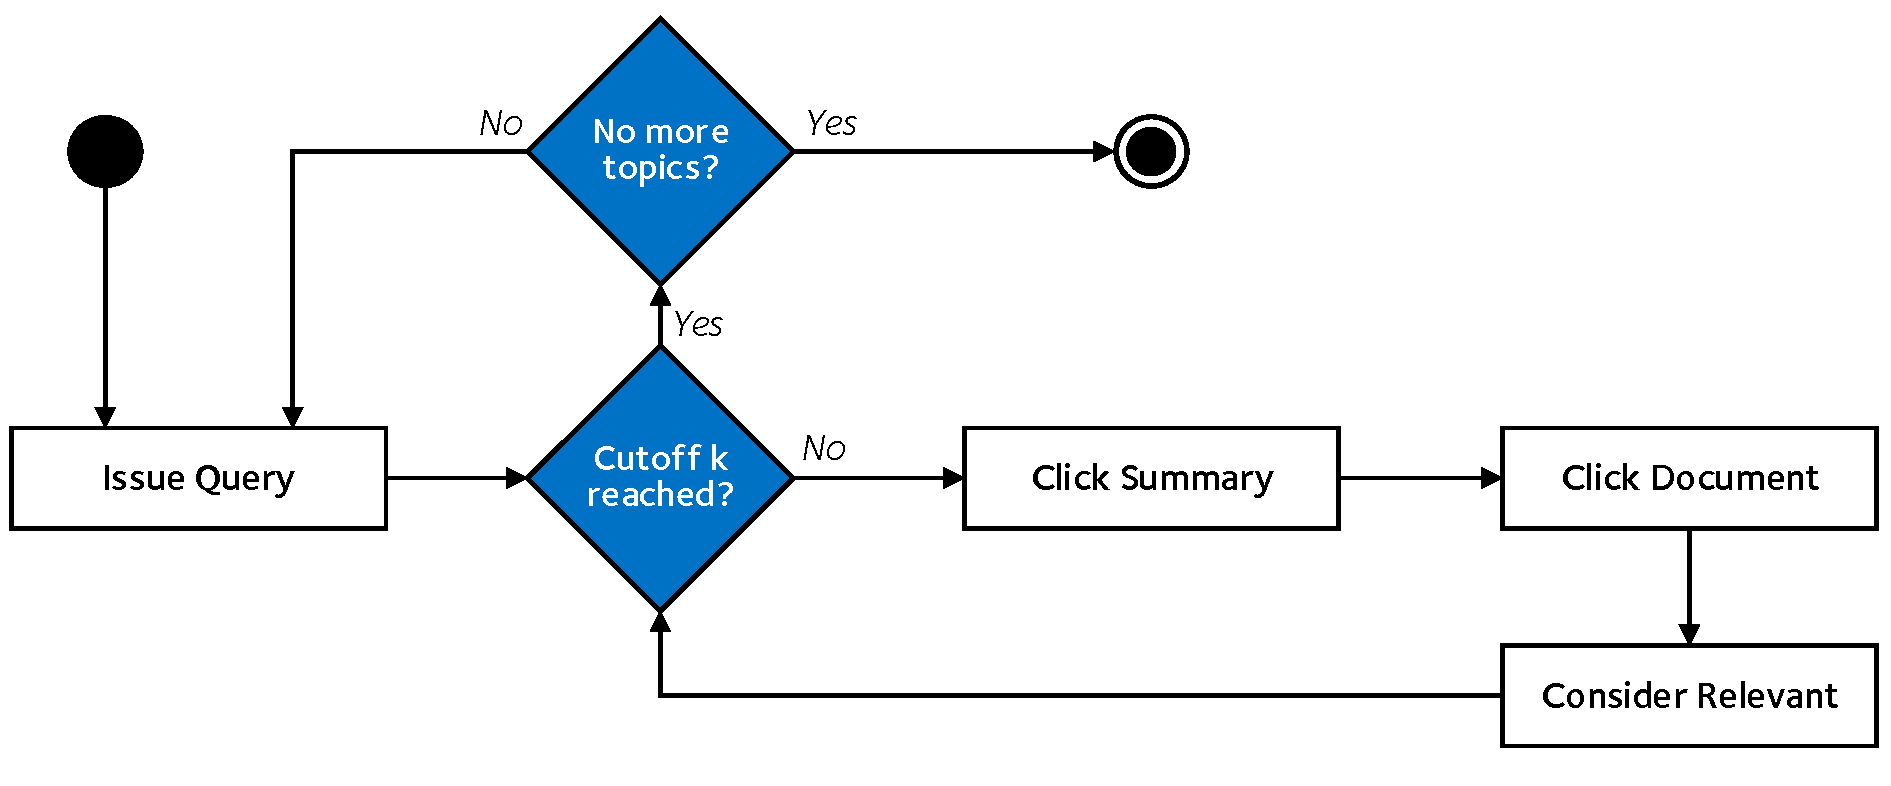
\includegraphics{figures/ch3-trec.pdf}}
    \caption[The TREC-style user model]{A basic flowchart of the user model typically encoded within TREC-style experimentation. Users subscribing to this model will issue a query – typically the title of a topic – and then proceed to examine results to some fixed depth, \emph{k}.}
    \label{fig:trec_model}
\end{figure}

A basic flowchart of the user model is presented in Figure~\ref{fig:trec_model}. With a given information need, a searcher (or system) will then translate that information need into some form of query -- from most TREC tasks, the title of a topic is used (as discussed in Section~\ref{sec:ir_background:basics:cranfield}). The query is then issued to the underlying retrieval engine, and a set of results are then returned. From this point on, the process, as alluded to above, is \emph{batch-like} in nature. Every result summary presented is `clicked', with the document subsequently considered relevant, up to some cutoff at $k$. Typically for TREC-style experimentation, this cutoff will be $k=1000$. Once this process has been completed, the next query will be issued to the underlying retrieval engine, until the list of queries have been exhausted. Once this process has been completed, the list of documents considered relevant to the information need (i.e. all $k$ documents) are passed to the evaluation stage of the Cranfield model (refer to Figure~\ref{fig:ir_cranfield}), where the various evaluation measures that are to be used can be calculated.

The question one should ask considering this TREC-style user model is: \emph{is this model particularly realistic?} Arguments can obviously be made for and against such a model, but the general consensus in the~\gls{acr:ir} community is that it is \emph{not} particularly representative of a searcher in real life, regardless of the search task. A number of strong assumptions are made of the behaviour of the searcher, namely that:

\begin{itemize}
    \item{a single query is issued to address a given information need;}
    \item{a searcher subscribing to this model will \emph{always} examine to a fixed depth in the presented results (their \emph{stopping behaviour}); and}
    \item{a searcher will always consider an item presented to him/her as relevant to their information need.}
\end{itemize}

These assumptions have over the years been proven to be largely unrealistic through empirical evidence. For example, searchers will often adapt their stopping behaviour depending upon the quality of the list of results presented.~\cite{borlund2003iir_model} also puts forward the notion that the model does not consider a searcher's \emph{dynamic information needs}. Here, his or her understanding of a particular topic will evolve over time as content is examined and their mental model evolves. The TREC-style model of search considers that the only point at which a searcher `learns' is at the querying stage.

While deficient in terms of considering a searcher's behaviours, the TREC-style user model has worked well for the batch-style experimentation that is typically employed at evaluation forums. Indeed, the model has been demonstrated as an effective means for evaluating the effectiveness when considering system sided research. Next, we discuss what advancements have been achieved in developing the notion of a user model of search further.

\subsubsection{Simple Searcher Models}
A number of studies have proposed more complex (and arguably more realistic) models of the search process, encapsulating a greater number of concepts within them. While no definitive line of research exists that demonstrates these advancements, closer examination of the relevant publications yields a series of developments.

One of the major limitations of the TREC-style model of search is the restrictive definition of what is regarded as a search session, with a \emph{single query} issued to address the underlying information need of the searcher. The search process however is inherently interactive~\citep{baskaya2013behavioural_factors}, with a searcher potentially issuing multiple queries (perhaps through query reformulations) as he or she accrues utility from the search results presented~\citep{ingwersen2005theturn}. To this end, seminal work by~\cite{baskaya2013behavioural_factors} presented an explicit, revised model of the interactive search process that improved on the definition of \emph{interactive}. Improvements over the TREC-style model included the following three key additions:

\begin{itemize}
    \item{the ability to \emph{separately judge snippets} presented on a~\gls{acr:serp} from the associated document;}
    \item{permitting a searcher subscribing to this model to \emph{stop at a variable depth on the~\gls{acr:serp},} avoiding fixed depth stopping behaviours as was typically employed in models of search; and}
    \item{on a related note, permitting a searcher to issue \emph{multiple queries} for the same information need during a search session.}
\end{itemize}

These improvements are demonstrated in a flowchart, illustrated in Figure~\ref{fig:baskaya_model_flow}. As can be seen from the flowchart, the typical \emph{browsing model} components (e.g. inspecting a document for relevance) as per~\cite{carterette2011models} is also integrated with \emph{query generation} and \emph{utility accumulation}, allowing a searcher to issue multiple queries, and gain utility from examining content. This, in addition to the three key additions list above, are detailed below.

\begin{figure}[t!]
    \centering
    \resizebox{1\hsize}{!}{
    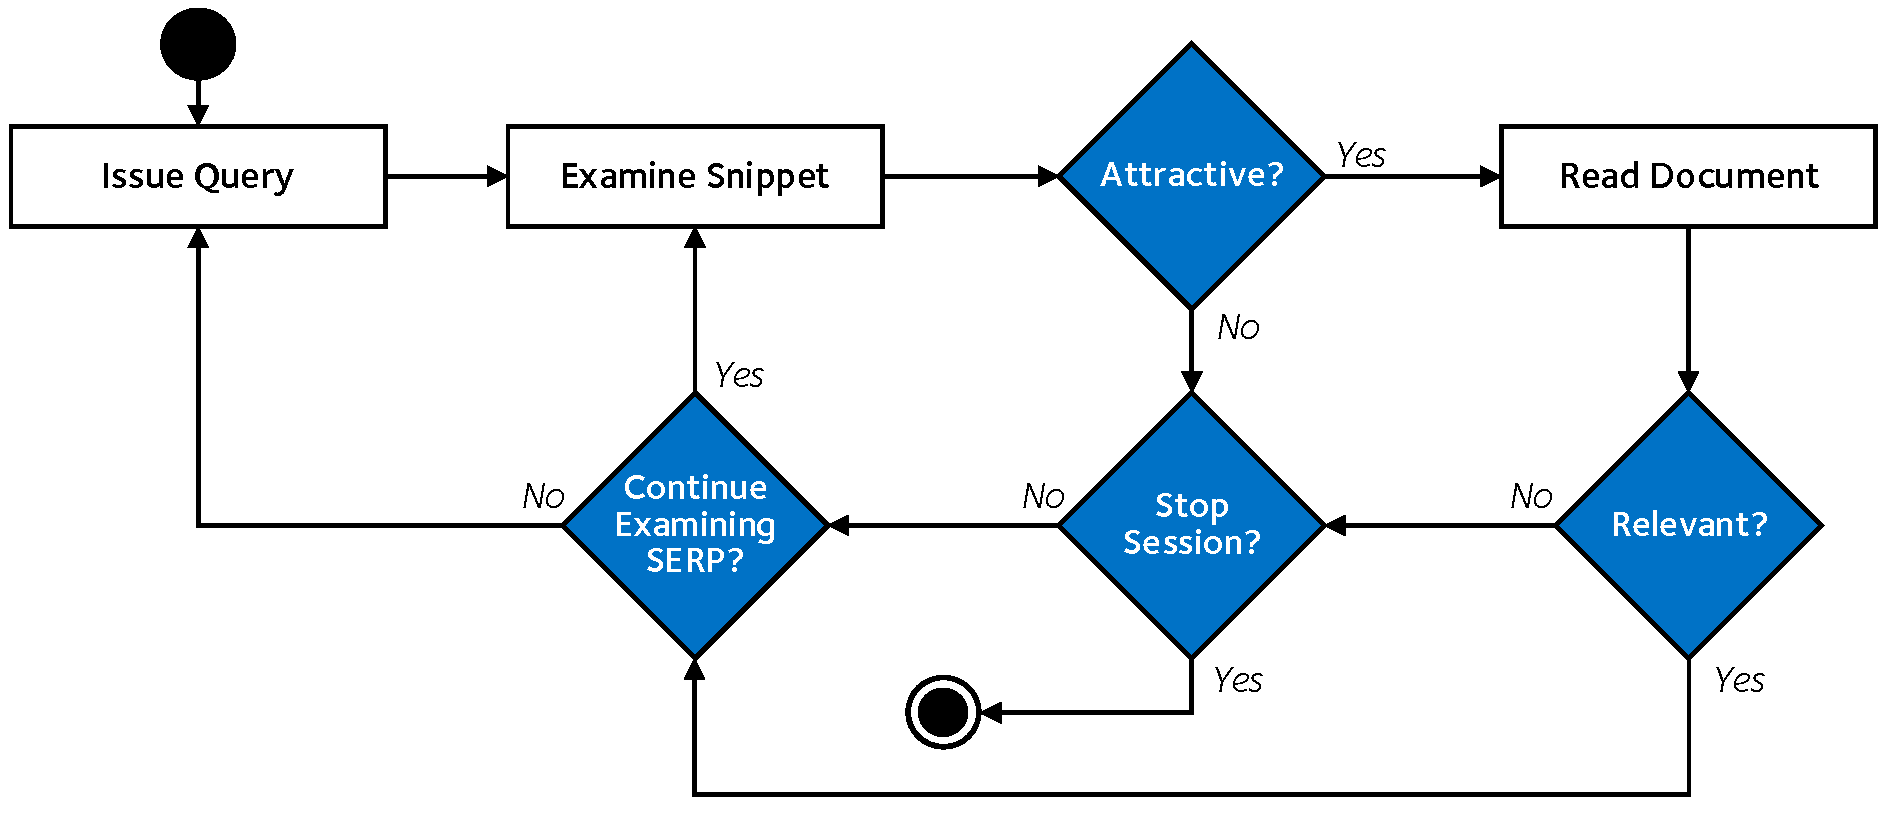
\includegraphics{figures/ch3-baskaya_flow.pdf}}
    \caption[Flowchart of the search process by~\cite{baskaya2013behavioural_factors}]{The user search model, as outlined by~\cite{baskaya2013behavioural_factors}. Adapted from the version of the model illustrated later in Figure~\ref{fig:baskaya_model}, this flowchart illustrates the main processes, decisions and interaction flow that an individual subscribing to this model will follow.}
    \label{fig:baskaya_model_flow}
\end{figure}

Judging snippets separately from the associated documents could be regarded as a major development in user models. Snippets can be generated via a variety of different means, with approaches typically \emph{query biased} in contemporary search engines~\citep{tombros1998query_biased}. As such, what may look like a snippet that is \emph{attractive} enough to explore further could potentially lead to a document that is in actuality not considered to be relevant. This is a clear development from the TREC-style approach that assumes all snippets (and associated documents) are relevant to the given information need.

Effectively modelling stopping behaviour is also important to providing a more realistic model of the search process. The addition of decision points allowing a searcher to judge the attractiveness of a snippet, or the relevancy of a document, provide natural locations for stopping decision points. \emph{Given this snippet looks unattractive and therefore not useful to satisfying my information need, should I stop examining the results presented to me on this~\gls{acr:serp}?} As an example, a searcher may issue a query that returns very few relevant documents. Once a few snippets and/or documents have been examined, he or she will then conclude that the issued query was unsuccessful, and that they would be essentially wasting their time examining more content on the present~\gls{acr:serp}. In this case, issuing a reformulated query would be a better course of action.

This intuition has been confirmed by empirical analysis, where~\cite{azzopardi2011economics} demonstrated that simulated searchers examined significantly fewer documents when the underlying search engine failed to retrieve any relevant material in the top ten results, in contrast to when it did. Thus, searchers are inherently adaptive, with their behaviours conditions on the quality of the ranked lists that they interact with. This provides a justification for including these additional stopping decision points.

Indeed, as previously discussed~\cite{azzopardi2011economics} simulated the behaviour of searchers using economic grounding to explain their observed behaviours. This led to the development of \emph{Search Economic Theory,} which we briefly discuss in more detail in Section~\ref{sec:stopping_background:models:theoretical:other}. The model employed by~\cite{azzopardi2011economics} was largely the same as that demonstrated in Figure~\ref{fig:baskaya_model_flow}, but without the addition of examining snippets in isolation from their complete document counterparts. Similar models have also been demonstrated by~\cite{yilmaz2010browsing_utility},~\cite{carterette2011models}, and more recently~\cite{zhang2017simulation_model}.

A further explicitly defined user model was proposed by~\cite{thomas2014modelling_behaviour}. This model, illustrated, again with a flowchart in Figure~\ref{fig:thomas_model}, essentially encapsulates the same principles as the previously described models: given an information need, a searcher will issue one or more queries, and examine a varying number of result summaries and documents. Also included is a form of utility accumulation model, that considers the utility obtained from a result summary $s_i$ and the relevancy judgement of a document, $r_i$. An addition to this model is the inclusion of an additional step at the beginning of the search session, where a searcher has the ability to \emph{select a search engine}.

\begin{figure}[t!]
    \centering
    \resizebox{1\hsize}{!}{
    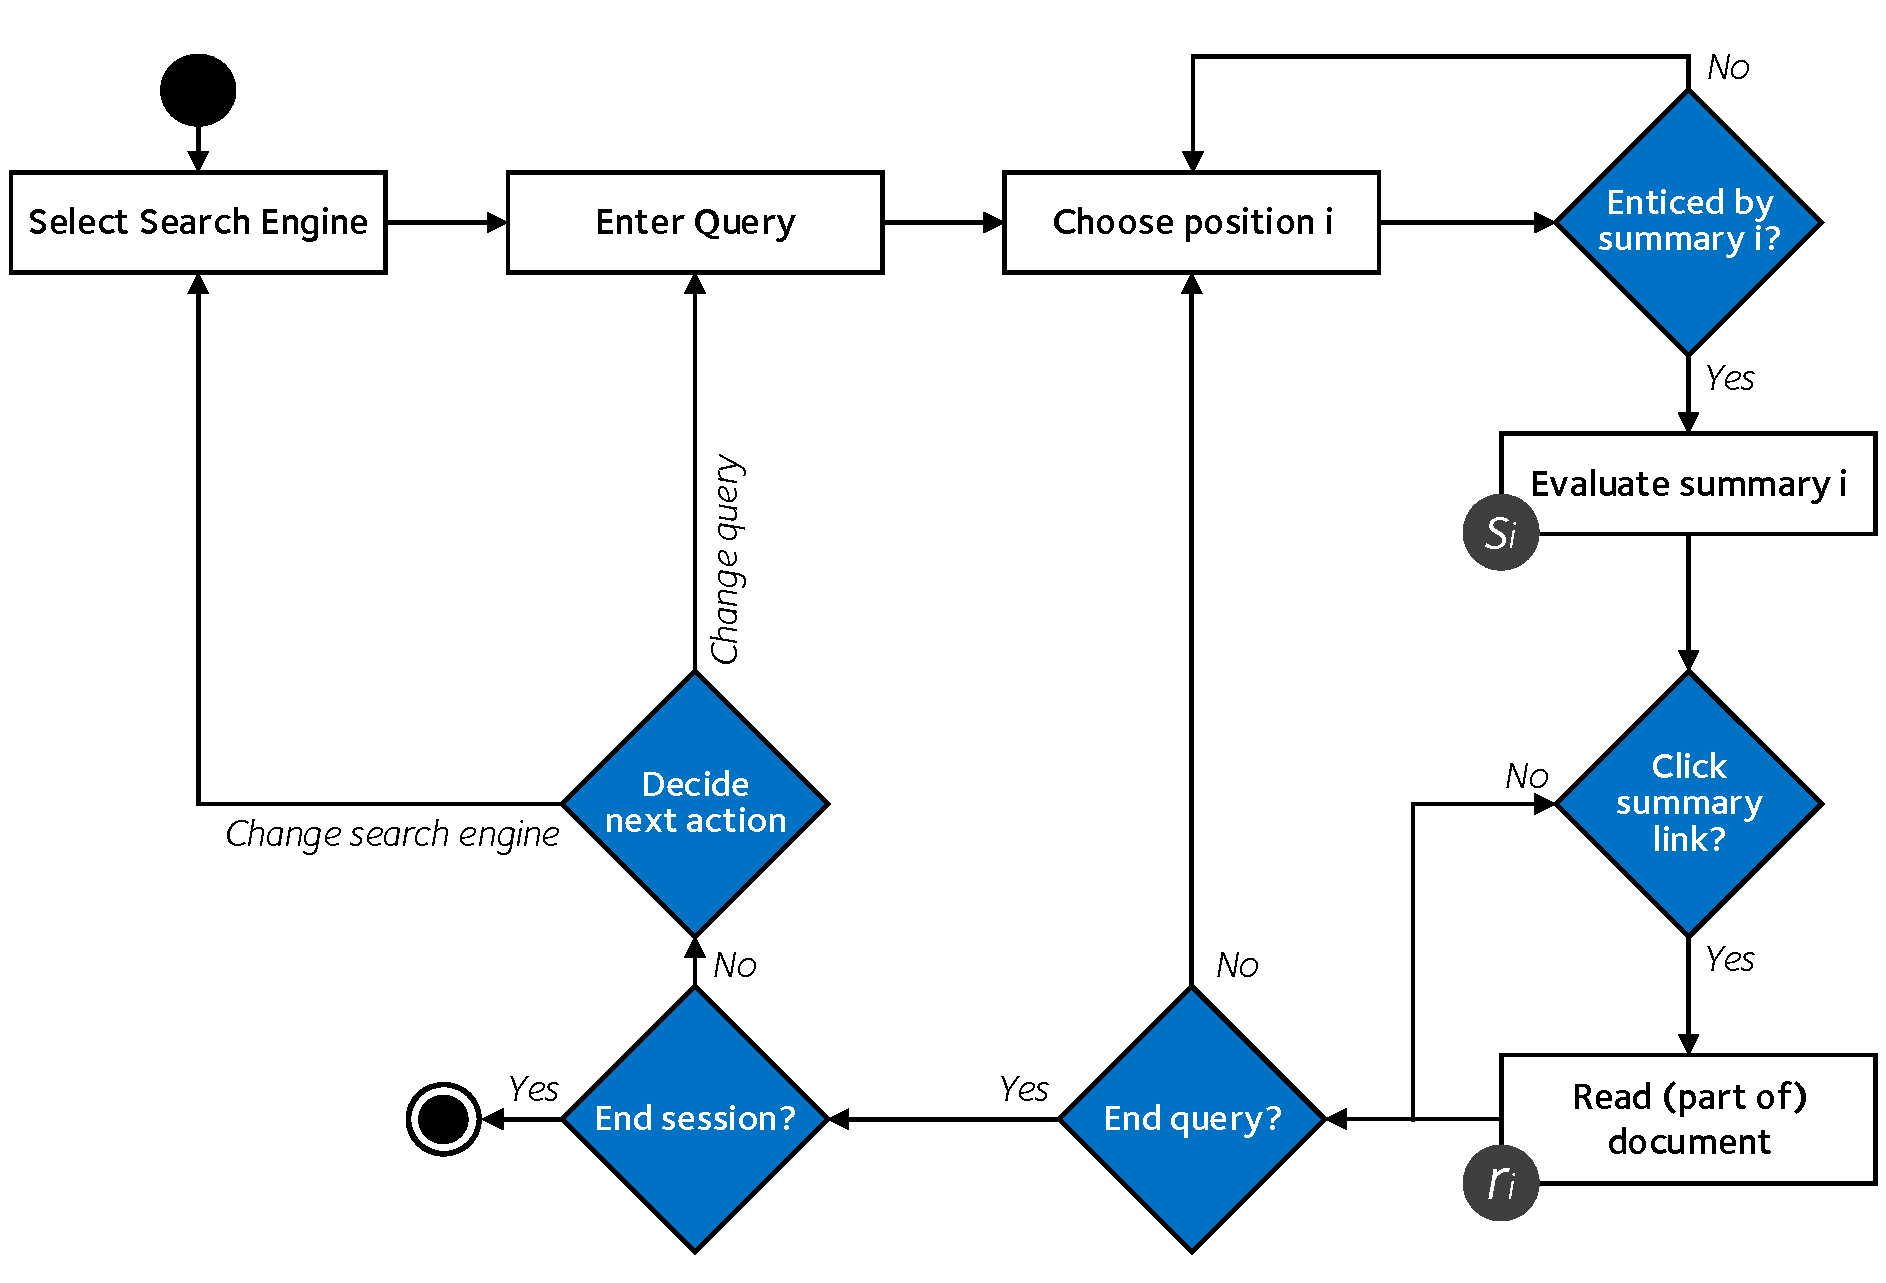
\includegraphics{figures/ch3-thomas.pdf}}
    \caption[Model of the search process by~\cite{thomas2014modelling_behaviour}]{A model of the search process, considering the high-level processes undertaken by a searcher, as outlined by~\cite{thomas2014modelling_behaviour}. Figure adapted (with permission) from the authors of~\citealt{thomas2014modelling_behaviour}. \textcopyright~Paul Thomas, Peter Bailey, Alistair Moffat and Falk Scholer.}
    \label{fig:thomas_model}
\end{figure}

As these models are conceptual in nature, there are many different means by which one can instantiate such a model, and subsequently simulate the behaviours of a searcher. For example, a stopping heuristic could be operationalised in such a way that it could form a basis for one of the decision points in the model illustrated in Figure~\ref{fig:baskaya_model_flow} above. We discuss ways in which we instantiated these components in Chapter~\ref{chap:proposal}.

\noindent
\blueboxbold{Representing Models} These are represented as flowcharts, but depending upon the way in which you wish to implement the model, different approaches might be better. For example, the model by Baskaya is depicted in their work as a Markov model, as they were primarily concerned with the search process interactions with respect to a number of probabilities. This is illustrated in Figure~\ref{fig:baskaya_model}. This is also present in the work, as an example, by~\cite{tran2017markov_models}. Flowcharts provide a versatile means for representing a conceptual model, as the different activities and decision points are level abstracted, meaning that you can implement them how you wish.

\begin{figure}[t!]
    \centering
    \resizebox{1\hsize}{!}{
    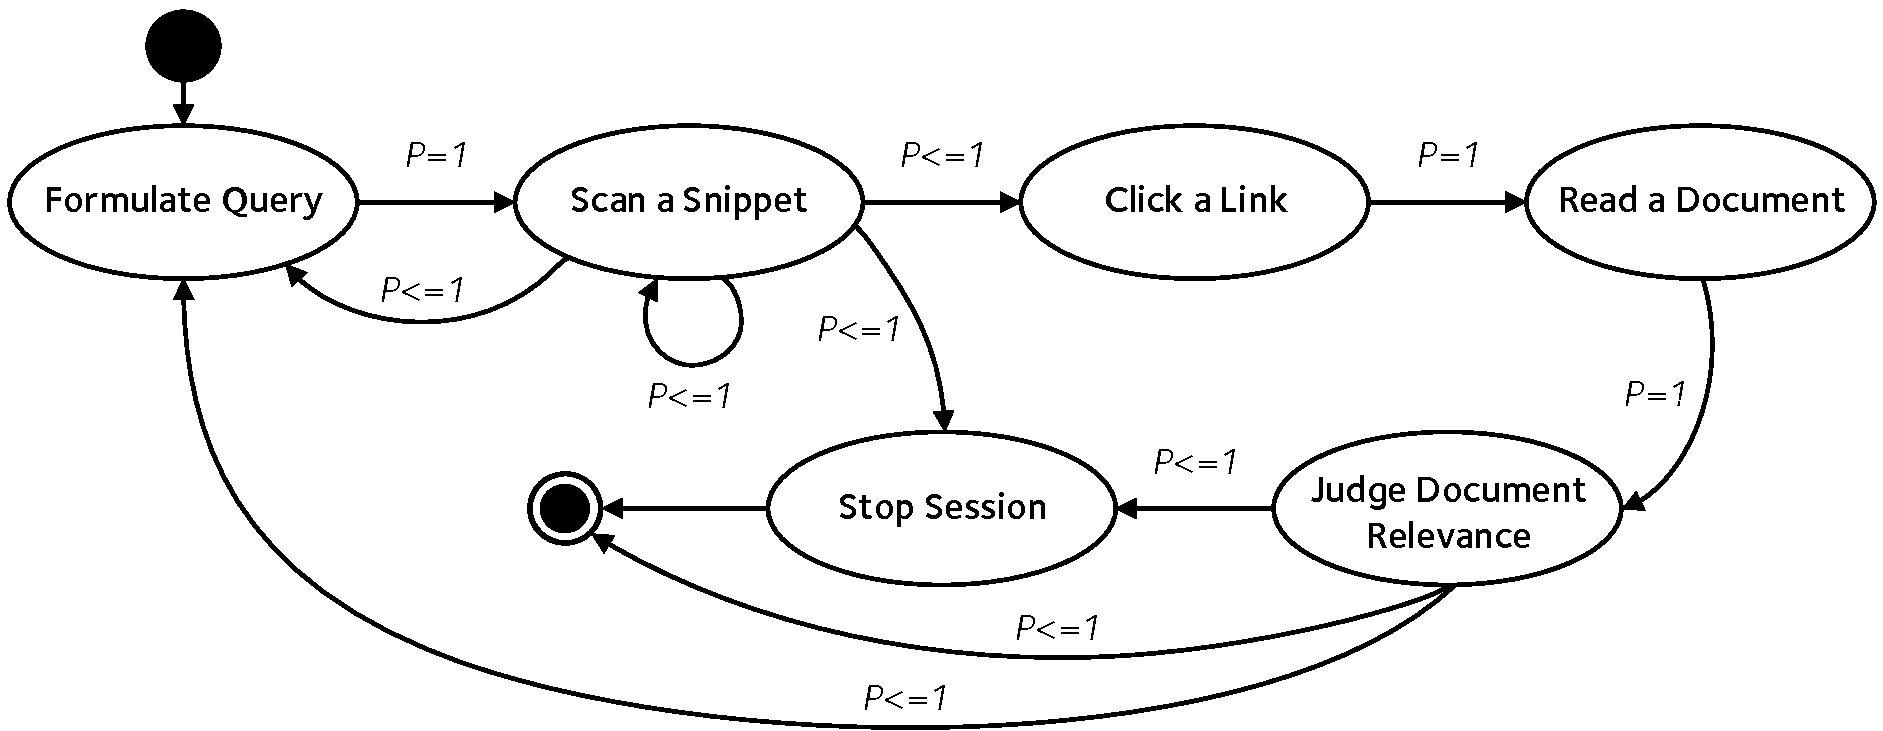
\includegraphics{figures/ch3-baskaya.pdf}}
    \caption[Markov model of the search process by~\cite{baskaya2013behavioural_factors}]{The user model of search, as outlined by~\citealt{baskaya2013behavioural_factors}. Represented as a Markov Model, the model considers six steps in all. Encoded within two of the steps are decision points that a user following this model must consider in order to continue. Figure adapted (with permission) from the authors of~\citealt{baskaya2013behavioural_factors}.}
    \label{fig:baskaya_model}
\end{figure}

\noindent
\blueboxbold{Considering Stopping Decision Points}
Considering the models described above, two clear \emph{stopping decision points} occur in every model presented. To demonstrate this, Figure~\ref{fig:model_two_points} illustrates an excerpt from a basic user model that highlights these two key stopping decision points. In the figure, decision point \blueboxbold{1} considers \emph{snippet level stopping} -- often referred to as \emph{query level stopping} in the literature.\footnote{In this thesis, we use the terminology \emph{snippet level stopping} to avoid potential confusion between this well defined stopping decision point, and a further one that we introduce in Chapter~\ref{chap:proposal}.} This stopping decision point addresses the issue of how deep a searcher should examine a ranked list of results presented to him or her on a given SERP. In addition to this, the second stopping decision point, \blueboxbold{2}, as demonstrated in Figure~\ref{fig:model_two_points}, considers wider \emph{session level stopping}. This stopping decision point permits a searcher to determine whether they have met their overall search goal, have run out of time, or have simply become exasperated with the lack of promising results. While these two key stopping decision points are discussed in more detail in Section~\ref{sec:proposal:stopping_points}, it should be noted that the heuristics defined in this section can be applied to snippet level stopping, session level stopping, or both.

\subsection{Theoretical Models}
In addition to the conceptual models described above, a number of different theoretical models have been defined in the literature that attempt to model the search process. In particular, we focus on~\gls{acr:ift} as a means for explaining a searcher's \emph{optimal stopping behaviour}. We also briefly discuss other competing theoretical models of search interactions.

\begin{figure}[t!]
    \centering
    \resizebox{1\hsize}{!}{
    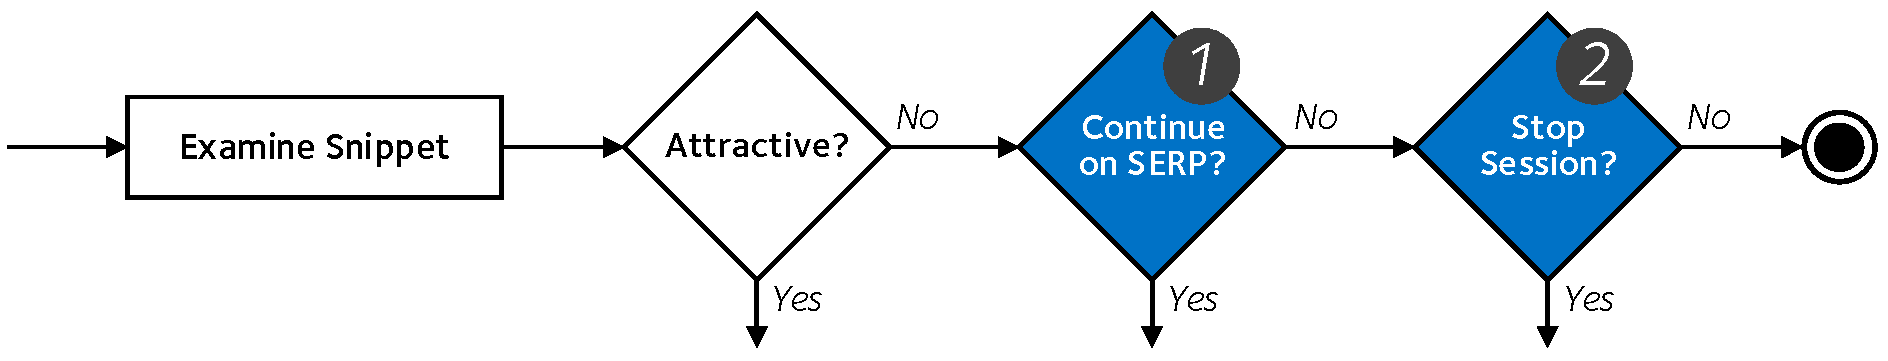
\includegraphics{figures/ch3-two_points.pdf}}
    \caption[Two main stopping decision points of the search process]{An excerpt from a wider user search model, demonstrating two key, established stopping decision points commonly discussed in the literature. These are highlighted in the illustration as {\color{dmax_lightblue}blue} diamonds. The two points consider \blueboxbold{1} \emph{snippet level stopping} (often called \emph{query level stopping}), and \blueboxbold{2} \emph{session level stopping}.}
    \label{fig:model_two_points}
\end{figure}

\subsubsection{Information Foraging Theory}\label{sec:stopping_background:models:theoretical:ift}
A well known conceptual model in the field of information seeking is the so-called \emph{Berry Picking model}, as proposed by~\cite{bates1989berry_picking}. As shown in Figure~\ref{fig:berry_picking}, this model considers searchers looking for information to be analogous to \emph{foragers} scavenging for food in the wild. In the model, foragers are looking for the juiciest and ripest berries on a number of different \emph{patches}, or bushes. The juiciest and ripest berries offer the highest levels of gain, or utility -- picking these berries help the forager maximise their level of \emph{gain.} Switching context, a searcher forages for information, picking the most relevant (or, if you will, juiciest) documents that help them maximise their gain, and in turn satisfy their information need.

While the Berry Picking model is an intuitive and simple model to understand, its highly descriptive nature does not provide an explanation regarding the behaviour of the forager. \emph{How long should a forager spend examining this berry bush?} This question cannot be answered as such by the model, but~\cite{bates1989alluding} in a later publication does allude to the fact that searchers could weigh up the costs and benefits in order to decide what to do next.

Theories do however exist that attempt to explain the behaviour of a searcher when \emph{foraging} for information. Initial attempts by~\cite{russell1993sense_making} and~\cite{sandstrom1994optimal_foraging} demonstrated that \emph{Optimal Foraging Theory}~\citep{stephens1986foraging_theory} could be potentially used to model the search process. This led to the development of~\gls{acr:ift}, proposed by~\cite{pirolli1999ift}. The theory provides an explanation as to how information foragers will behave, and as such, also provides a rationale as to how they will \emph{stop.}~\gls{acr:ift} is extensively used in this thesis as a theoretical underpinning to several hypotheses. It also provides a stopping heuristic that we outline later in this section.

\noindent
\blueboxbold{Diet, Patches and Scent}~\gls{acr:ift} is comprised of three main models: the \emph{information diet model}, concerning \emph{what} information is consumed; the \emph{information patch model}; and the \emph{information scent model.} With the work on this thesis considering the patch and scent models, we now provide an explanation of these two models.

\begin{figure}[t!]
    \centering
    \resizebox{1\hsize}{!}{
    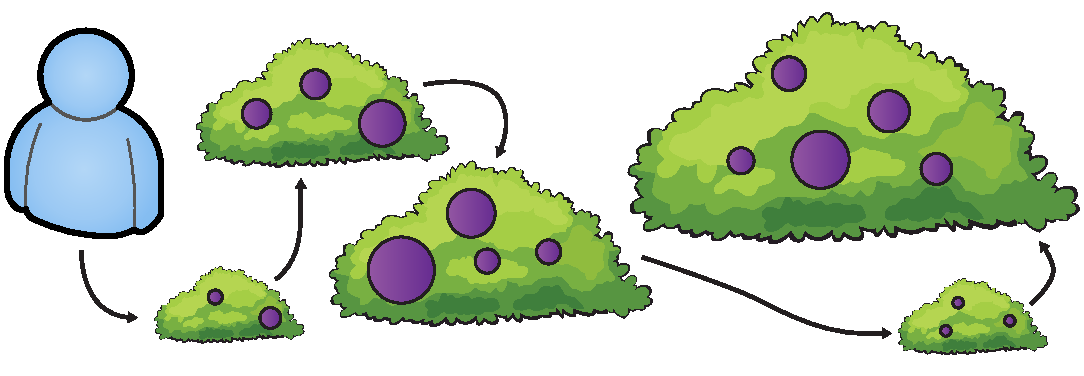
\includegraphics{figures/ch3-berry_picking.pdf}}
    \caption[The Berry Picking Model~\cite{bates1989berry_picking}]{The \emph{Berry Picking Model,} defined by~\cite{bates1989berry_picking}. A forager traverses through numerous bushes to pick the juiciest berries for his or her consumption. The model is high level and conceptual in nature, and thus does not provide any justification for \emph{how} or \emph{why} foragers search for the juiciest berries.}
    \label{fig:berry_picking}
\end{figure}

Central to~\gls{acr:ift} is the notion of a \emph{patch}, as per the patch model. In the wild, a patch is modelled as an area of land with a degree of potential gain (food) that can be acquired by foraging through said patch. The \emph{between patch time} is the amount of time a forager spends moving towards a patch, and the \emph{within patch time} is the time spent within the patch, examining its contents.

With~\gls{acr:ift}, a patch can be modelled in a variety of ways. However, as outlined by~\cite{azzopardi2015theories}, the generally agreed approach to model a patch in terms of information seeking is to consider it as a~\gls{acr:serp}. In this model, moving between a patch is akin to \emph{issuing a query,} and thus incurs a cost (between patch time), and staying within a patch is the same as assessing result summaries on the presented~\gls{acr:serp} and their associated documents, with each summary and/or document taking a certain amount of time to process (within patch time). The patch model essentially predicts how long an information forager should stay in a patch, before moving onto the next patch.

Given a series of patches, however, how does a forager deduce which one he or she should \emph{enter} next, and examine in closer detail? This is described by the information scent model, and encapsulates a currently active area of research. Figure~\ref{fig:patch_model} graphically illustrates the scent of a patch in action -- given two patches as depicted in the illustration, what patch will the forager travel to next? Following the scent, or \emph{cues} on the ground next to him, the forager observes that the paw prints to the first patch are more prevalent, and thus will venture to that patch first. Like foragers in the wild, information foragers will observe a series of \emph{proximal cues} presented to them on a~\gls{acr:serp}, such as hypertext links, document titles, snippet text and thumbnails to locate information~\citep{pirolli1995ift, pirolli1999ift, chi2001information_scent, oltston2003scenttrails, pirolli2007ift}. In the context of news search, cues were examined by~\cite{sundar2007news_scent}. Here, cues such as the source of an article were shown to have a powerful effect on the perception of said article.

\begin{wrapfigure}[12]{r}{0.45\textwidth}
    \begin{center}
    \vspace*{-10mm}
    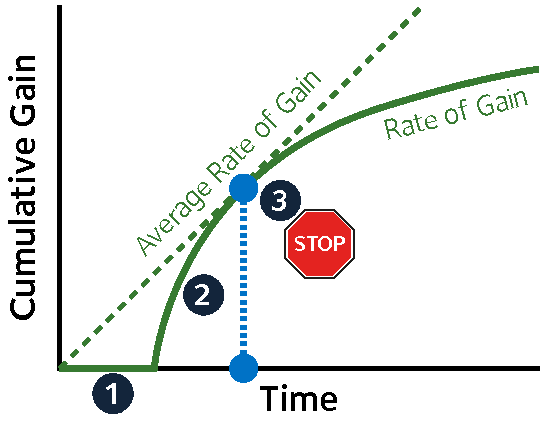
\includegraphics[width=1\textwidth]{figures/ch3-ift_stop.pdf}
    \end{center}
    \vspace*{-4mm}
    \caption[\gls{acr:ift} Stopping Heuristic]{The~\gls{acr:ift} stopping heuristic. The searcher should stop when the rate of gain (solid {\color{dmax_green}green} line) no longer outperforms the average rate of gain (dotted {\color{dmax_green}green} line).}
    \label{fig:ift_stopping}
\end{wrapfigure}

If these cues provide a rationale as to what leads to a promising scent trail, it follows that scent, in combination with patches, provides a rationale as to when a searcher will stop examining a set of results~\citep{pirolli1999ift, wu2012dc, wu2014information_scent}. For example, as demonstrated in Section~\ref{sec:stopping_background:user_studies},~\cite{wu2014information_scent} demonstrated that a searcher would forage to greater depths if the~\gls{acr:serp} appears to contain many relevant items. This trend was also observed by~\cite{card2001scent_graphs}, who found that when navigating through webpages, searchers were more likely to leave when the information scent began to decline.

\begin{figure}[t!]
    \centering
    \resizebox{1\hsize}{!}{
    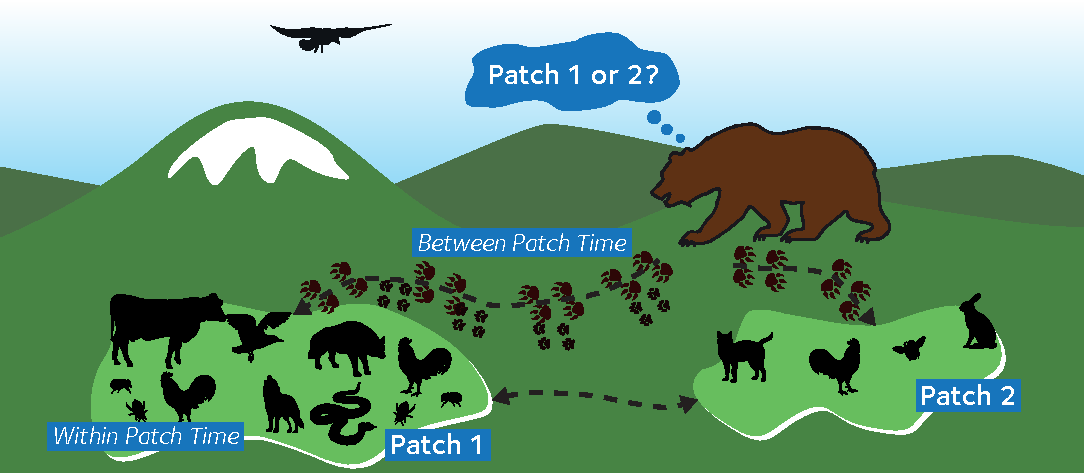
\includegraphics{figures/ch3-patch.pdf}}
    \caption[The Patch Model]{A graphical depiction of the \emph{Patch Model}, part of \emph{Information Foraging Theory.} When presented with two patches, each containing food that can be represented as gain, what patch should our forager choose first — patch 1 or 2?}
    \label{fig:patch_model}
\end{figure}

\noindent
\blueboxbold{The~\gls{acr:ift} Stopping Heuristic}
Given a patch with a scent, how can one deduce \emph{when they should stop?} Like all theories,~\gls{acr:ift} makes some key assumptions from which we can deduce behavioural characteristics of a forager. These assumptions are that a forager will:

\begin{itemize}
    \item[\emph{(i)}]{enter a patch with what appears to be the highest yield first; and}
    \item[\emph{(ii)}]{attempt to maximise their gain per unit of time.}
\end{itemize}

Given these assumptions, one would now be able to answer the question posed in the graphical illustration of patches in Figure~\ref{fig:patch_model}. With the better scent, and greater volume of potential energy to be gained, the first patch is the obvious answer that a forager would answer to the question: \emph{which patch should I explore first?}

In addition, the assumptions provided above allow us to begin formulating a stopping heuristic based upon the \emph{optimal behaviour} of a forager. The \emph{Maximum Marginal Theorem} by~\cite{charnov1976mvt} states...

\begin{quote}
    \emph{``...that a forager should remain in a patch so long as the slope of the gain function is greater than the average rate of gain in the environment.''}
    \attrib{\cite{pirolli1999ift}}
\end{quote}

The Maximum Marginal Theorem implies that is a forager is within a patch that initially looked promising, yet is yielding a rate of gain less than the \emph{average rate of gain,} he or she should abandon the patch and then move to another one. In the context of information seeking, this would imply a query reformulation. Conversely however, a forager who has found himself or herself in a patch yielding gain at a rate \emph{greater} than the average rate of gain would be best advised to stay within said patch. This is graphically illustrated in Figure~\ref{fig:ift_stopping}, where the \emph{gain curve} for a forager is highlighted in {\color{dmax_green}green.} In addition, the plot illustrates: \emph{(1)} the between patch time, where the forager is not acquiring any gain; \emph{(2)} the within patch time, where the forager is examining the~\gls{acr:serp} and associated documents; and \emph{(3)} the optimal stopping point, based upon the Maximum Marginal Theorem. Graphically, this is best described as the point at which the tangent to the curve (from the origin) touches the gain curve. From this point onwards, the rate of gain decreases, meaning that the forager is receiving ever increasing diminishing returns for the investment in examining content on the current patch.

\subsubsection{Other Theoretical Models of Search}\label{sec:stopping_background:models:theoretical:other}
It is important to acknowledge that apart from~\gls{acr:ift}, other competing theoretical models of search exist. While we do not discuss them in any great depth, we do in this section provide a brief overview of the work undertaken that led to each, along with references to both. We consider an economics based theory, \emph{Search Economic Theory (SET)} outlined by~\cite{azzopardi2011economics}, and the \emph{Interactive Probability Ranking Principle (iPRP)} as outlined by~\cite{fuhr2008iprp}. With many of the contributions in this thesis utilising~\gls{acr:ift}, we limit the discussion provided for SET and the iPRP.

\noindent
\blueboxbold{Modelling Stopping Behaviours}~\cite{azzopardi2015theories} conducted an extensive empirical study comparing the two competing theoretical models of search listed above, in tandem with~\gls{acr:ift}. Their goal was to develop a model for ad-hoc topic retrieval using each of the three approaches, in order to determine what predictions make about search behaviours, and show the relationships and differences between the three approaches. The authors noted that while the three competing models took different perspectives on modelling searcher interactions, their mathematical proofs led to similar hypotheses regarding searcher behaviours -- including stopping behaviours.

\noindent
\blueboxbold{Cost/Benefit Decision Making} Cost-benefit and other decision making tools form the foundations of both SET and the iPRP, and indeed are nothing new to the field of~\gls{acr:ir}. For example, the \emph{Probability Ranking Principle (PRP)} proposed by~\cite{robertson1977prp} and discussed in Section~\ref{sec:ir_background:basics} is an example of a prior application of such a framework, and offered advancements in how~\gls{acr:ir} systems ranked documents. Indeed, the PRP has been recently revised by~\cite{fuhr2008iprp} to consider a series of interactions that take place during a~\gls{acr:iir} session. This high level, generalisable model accounts for the different costs and benefits that are associated with particular \emph{choices} when ranking a series of documents.

\noindent
\blueboxbold{\gls{acr:ir} from an Economic Perspective}~\cite{varian1999economics} outlined three directions in which economics could be of use when considering search:

\begin{itemize}
    \item[\emph{(i)}]{obtaining a better estimate of the probabilities of relevance;}
    \item[\emph{(ii)}]{applying \emph{Optimal Search Behaviour}~\cite{stigler1961economics} to~\gls{acr:ir}; and}
    \item[\emph{(iii)}]{examining the economic value of information using \emph{consumer theory}, where \emph{``a consumer is making a choice to maximise expected utility of minimise expected cost''}~\citep{varian1999economics}.;}
\end{itemize}

Several studies have tackled the first two directions (refer to~\cite{birchler1999information} and more recently~\cite{wang2009economics} for examples). However, with regards to the third option, \emph{production theory}~\cite{varian1987intermediate} was employed by~\cite{azzopardi2011economics} to model the interactive search process. This led to the development of SET, which has been subsequently revised in future publications to include more complex components of the search process, such as snippet examinations -- including the associated costs and benefits from such a process (refer to~\cite{azzopardi2014economics}).

\section{Chapter Summary}
In this chapter, we have provided an extensive overview of how stopping behaviours have been examined in~\gls{acr:iir}. In addition to this, we have examined a variety of different user models that attempt to capture the search process.

In particular, we have detailed a number of different stopping heuristics that have been proposed in the literature. These heuristics are the attempts of researchers to attempt and capture what is described as a searcher's feeling of what they have found is \emph{``good enough''}~\citep{zach2005enough_is_enough}. Indeed, we also provided a review of the literature concerning user studies examining searcher stopping behaviours. Many of these studies discovered that searchers are simply unable to articulate their behaviours, and found that a searcher stops when their internal stopping heuristics consider that what they have found is enough to satisfy them -- complying with the \emph{satisfaction stopping heuristic,} for example. However, these different internal stopping heuristics vary from person to person, with factors such as domain knowledge and external factors like time constraints affecting their behaviours~\cite{marchionini1995information_seeking}. As such, although several studies have been undertaken, examining stopping behaviours is a very difficult phenomenon to capture effectively.

Our discussion on user models also provided an overview of the different evolutions of model. These range from the basic TREC-style model of search up to the contemporary simple user models, capturing several additional activities and decision points, which provide a natural entry point for modelling searcher stopping behaviours. We also provided an overview of~\gls{acr:ift}, considering how this theory allows us to determine a searcher's optimal stopping behaviour.

With this outline of the current state-of-the-art, we now turn our attention to the contributions provided in this thesis. In the next chapter, we outline our updated user model of search, incorporating additional decision points for examining and modelling searcher stopping behaviours. We also detail how we \emph{operationalise} the aforementioned stopping heuristics, and turn them into a series of \emph{implementable stopping strategies.}











% - given you an outline of the basics of IR
% - and more system-sided IR
%
% - including a discussion on some of the various measures that are used
% - still very naive in terms of \emph{stopping behaviour}. i.e. assume fixed depths, typically naive about relevance.
%
% - so in this chapter, we begin to consider things from the central point of this thesis - stopping during search.
%
%
%
% - to this end, we in this chapter discuss:
%
% - a variety of different stopping heuristics
% - discuss the basic theories that can be used to explain one's stopping behaviour;
% - and explain the results from different user studies examining a searcher's stopping behaviour
%
% - we then take time to examine
%
% - some of the more complex models of search which are better able to capture stopping.
% 
% \section{Stopping Heuristics}\label{sec:stopping_background:heuristics}
%
% \section{User Studies}
% ryen white's expert stuff -- does he report stopping stuff?
%
% depth first vs breadth first??
%
% conceptual models (e.g. following on from TREC, we end up with...thomas, baskaya...), then move on to theoretical models
%
% like we mentioned in Ch2, in the different measures, we have different stopping rules encoded within them.
% e.g. Carterette's 2011 model.
%
% \section{Models of Search}
%
% \subsection{Conceptual Models}
% The Berry Picking Model
%
% \begin{figure}[t!]
%     \centering
%     \resizebox{1\hsize}{!}{
%     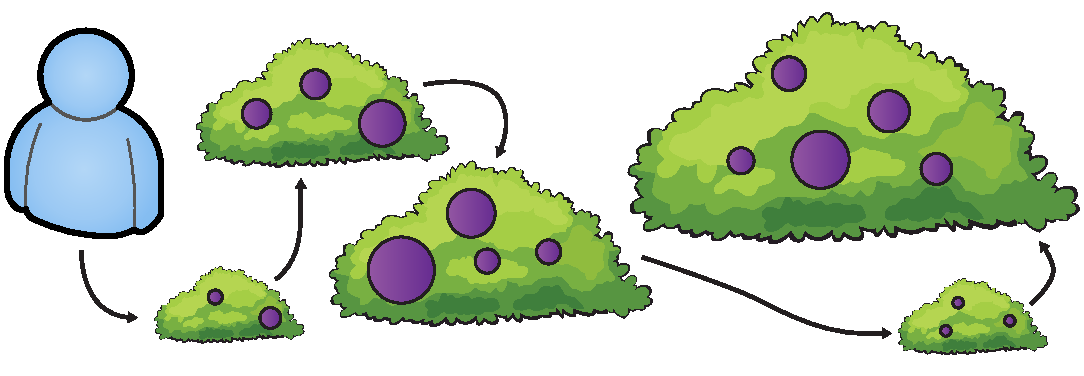
\includegraphics{figures/ch3-berry_picking.pdf}}
%     \caption[The Berry Picking Model~\cite{bates1989berry_picking}]{The Berry Picking Model, defined by~\citealt{bates1989berry_picking}.}
%     \label{fig:berry_picking}
% \end{figure}
%
%
% \subsection{Information Foraging Theory}
%
% \subsection{(Interactive) Probability Ranking Principle}
%
% \subsection{Search Economic Theory}
%
% \subsection{Simple TREC User Model}
%
% \subsection{Paul Thomas Model}
%
% \subsection{Feza Model}
%
% Need to illustrate that there is a development of the user model here.
%
% What about the attention model in ``Beyond ten blue links: enabling user click modeling in federated web search''?
%
% \begin{figure}[t!]
%     \centering
%     \resizebox{1\hsize}{!}{
%     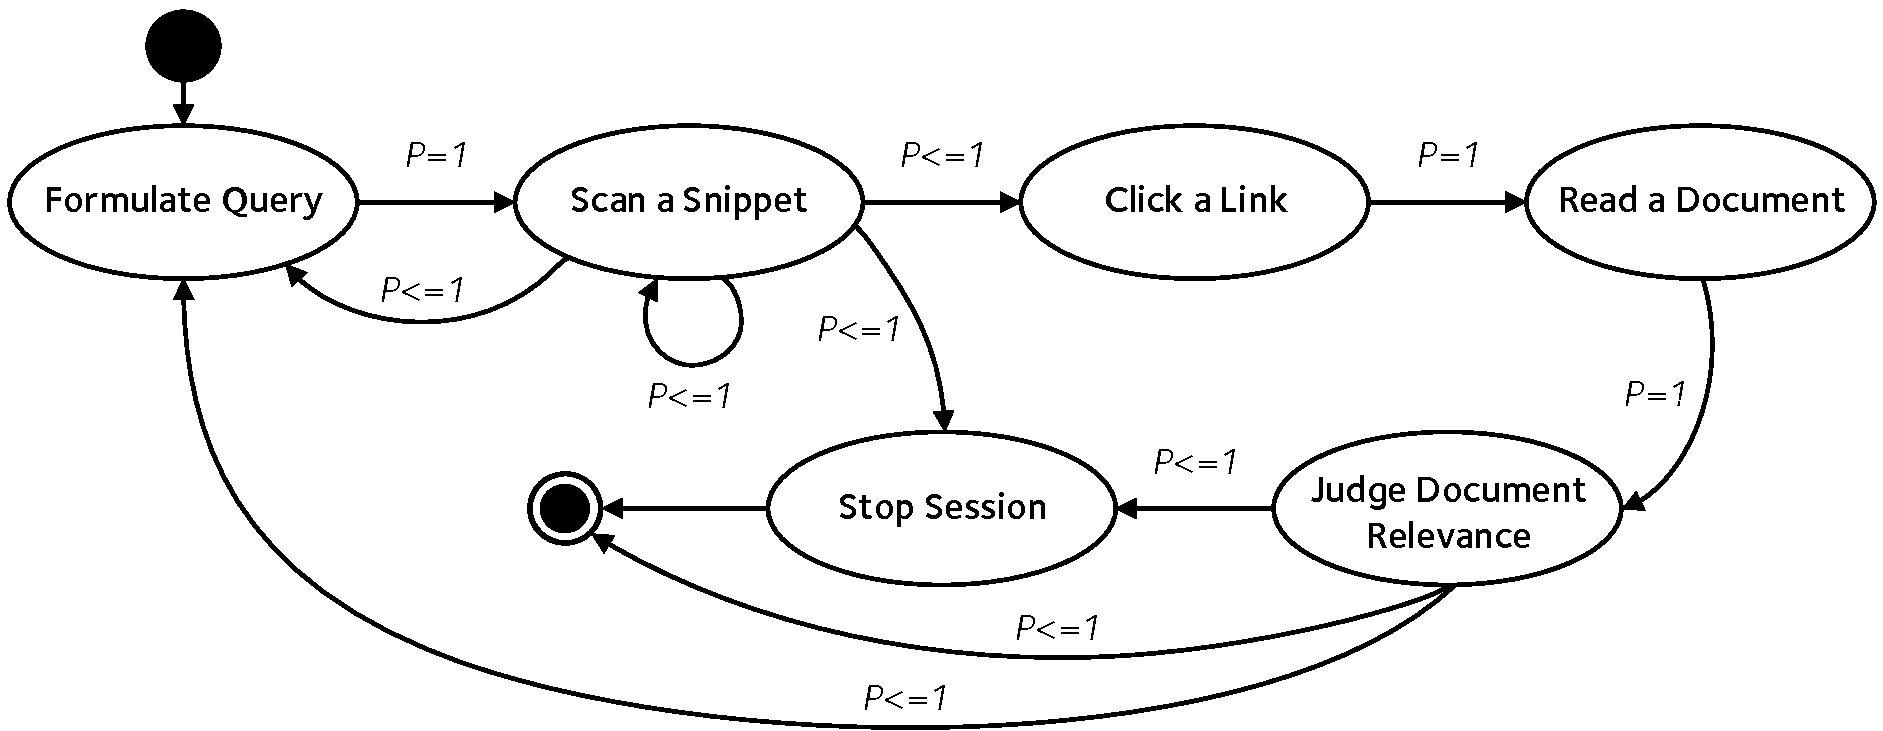
\includegraphics{figures/ch3-baskaya.pdf}}
%     \caption[Model of the search process by~\cite{baskaya2013behavioural_factors}]{The user model of search, as outlined by~\citealt{baskaya2013behavioural_factors}. Represented as a Markov Model, the model considers six steps in all. Encoded within two of the steps are decision points that a user following this model must consider in order to continue. Figure adapted (with permission) from the authors of~\citealt{baskaya2013behavioural_factors}.}
%     \label{fig:baskaya_model}
% \end{figure}
%
% \begin{figure}[t!]
%     \centering
%     \resizebox{1\hsize}{!}{
%     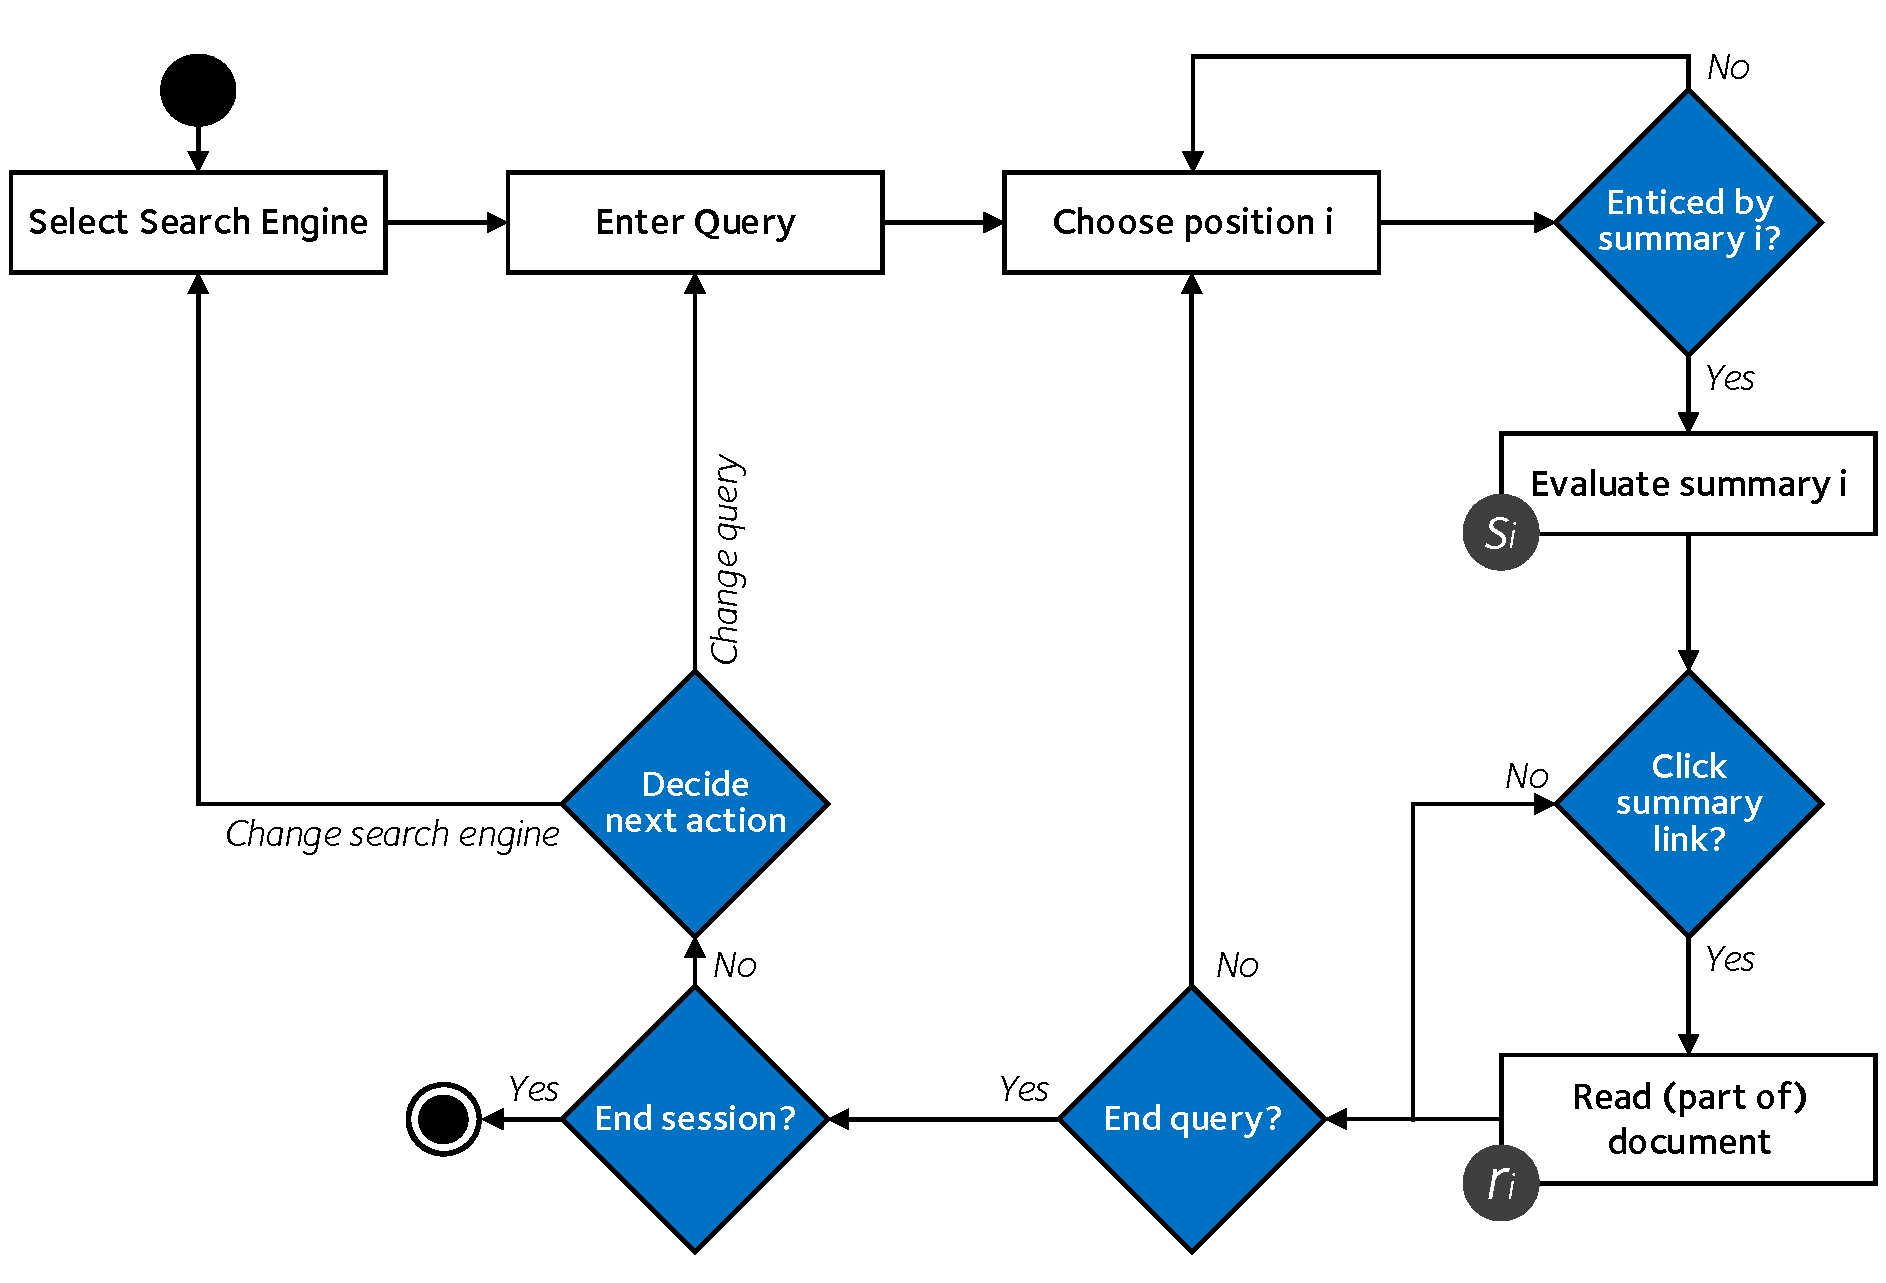
\includegraphics{figures/ch3-thomas.pdf}}
%     \caption[Model of the search process by~\cite{thomas2014modelling_behaviour}]{A model of the search process, considering the high-level processes undertaken by a searcher, as outlined by~\cite{thomas2014modelling_behaviour}. Also included are a number of decision points (represented as diamonds) that searchers must consider when following this model. Figure adapted (with permission) from the authors of~\citealt{thomas2014modelling_behaviour}. \textcopyright~Paul Thomas, Peter Bailey, Alistair Moffat and Falk Scholer.}
%     \label{fig:thomas_model}
% \end{figure}
%
%
% Refer to the following chapter for more information on how we extend these models to make them more realistic.
%
